\chapter{Procese}
\label{chapter:process}

Un proces este o aplicație ce se execută în sistemul de operare, folosind resursele sistemului, pentru a realiza o acțiune cerută de utilizator. Acțiunile utilizatorului pot fi să deschidă o pagină web, să creeze o imagine, să asculte o melodie. Utilizatorul face aceste acțiuni folosind aplicații precum un browser web, o suită Office, un player audio.

La nivelul sistemului de operare, aceste aplicații sau comenzi pornite de
utilizator sunt procese. Atunci când o aplicație sau un program rulează, spunem
că face acest lucru în contextul unui proces. Spunem despre procese că
\textbf{rulează} sau că \textbf{se execută} sau că \textbf{se află în execuție}.
Procesele sunt entități active care, atunci când rulează, folosesc resursele
sistemului: procesor, memorie, sistem de fișiere.

Înțelegerea proceselor este esențială pentru orice utilizator pentru a asigura
buna funcționare a sistemului; atunci când sistemul nu este responsiv, cauza
probabil este un proces care consumă excesiv resursele sistemului. Un
dezvoltator de aplicații va folosi cunoștințe despre procese pentru a proiecta
aplicații performante care să folosească cât mai eficient resursele sistemului.
Un inginer de sistem va monitoriza procesele sistemului pentru a se asigura de
buna funcționare a acestuia și pentru a preveni atacuri de securitate sau abuz
de resurse.

O parte dintre procese sunt pornite de la acțiuni ale utilizatorilor, precum
rularea unei aplicații grafice sau a unei comenzi. Numim aceste procese
\textbf{interactive} pentru că interacționează cu utilizatorul pe parcursul
rulării lor. Alte procese sunt pornite de sistem și nu interacționează cu
utilizatorul. Acestea au rol în gestiunea sistemului sau oferirea de servicii;
de exemplu conectarea la rețea în momentul în care există o rețea wireless
disponibilă sau actualizarea ceasului sistemului sau indexarea fișierelor pentru
căutare rapidă. Aceste procese sunt \textbf{neinteractive}. Le numim
\textbf{servicii} sau, pe Unix, procese \textbf{daemon}. Vom discuta mai în
detaliu în \labelindexref{Secțiunea}{sec:process:daemon}.

Unele aplicații pot fi compuse din mai multe procese. De exemplu, un browser
web precum Google Chrome pornește un proces pentru fiecare tab; un server web
care servește cereri în rețea poate avea mai multe procese care fac servirea; o
fereastră de terminal are un proces shell deschis pentru fiecare tab;
mai mult, într-o fereastră de terminal pot rula mai multe procese așa cum vom
vedea în \labelindexref{Secțiunea}{sec:process:foreground-background}.
Altfel spus, când folosim interfața grafică, o fereastră de aplicație care
rulează poate avea în spate mai multe procese. Sistemul de operare folosește
noțiunea de proces; este preocuparea dezvoltatorului de aplicații dacă o
aplicație folosește, când rulează, unul sau mai multe procese. \labelindexref{Figura}{fig:process:overview} este o perspectivă a proceselor și resurselor folosite de acestea.

\begin{note}[procese și cerințe]
Esențial este că orice aplicație care rulează în sistem, folosește unul sau mai multe procese pentru a satisface cerințele utilizatorului.
\end{note}

\begin{figure}[!htbp]
	\centering
	\def\svgwidth{0.5\textwidth}
	\includesvg{chapters/04-process/img/proc-overview.svg}
	\caption{Procese și resursele lor}
	\label{fig:process:overview}
\end{figure}

Pentru utilizator și sistemul de operare, procesele sunt necesare ca formă de
încapsulare. Un proces execută o anumită acțiune fără a afecta alt
proces. În general, procesele au resurse proprii oferite de sistemul de operare,
dar pot și partaja anumite resurse. Acest lucru este util pentru a realiza
acțiuni ce nu pot fi obținute cu un singur proces. De exemplu, un proces
descărcă un fișier video, alt procese îl convertește într-un format adecvat, alt
proces îl vizualizează. Vom vedea mai multe despre comunicarea și interacțiunea
între procese în \labelindexref{Secțiunea}{sec:process:operations}

Concret, sistemul de operare oferă:

\begin{itemize}
	\item izolare a resurselor proceselor, asigurându-se că, în mod normal,
		un proces nu poate accesa sau corupe resursele altui proces. În
		acest fel sistemul este menținut integru și fiecare proces se
		execută corespunzător.
	\item arbitrare a accesului la resurse partajate: dacă două sau mai
		multe procese accesează o resursă comună (de exemplu un fișier),
		atunci accesele trebuie să fie bine ordonate și, de exemplu, să
		nu suprascrie un proces informațiile celuilalt.
	\item mecanisme explicite de comunicare între procese: procesele
		comunică între ele pentru realizarea unei acțiuni mai complexe.
                Vom discuta în \labelindexref{Secțiunea}{sec:process:signal}, respectiv \labelindexref{Secțiunea}{sec:process:pipe} despre semnale și pipe-uri,
		două mecanisme de bază de comunicare între procese.
	\item comportament echitabil al proceselor, prin asigurarea că un proces
		nu utiliza prea multe resurse: un proces poate utiliza foarte
		multă memorie sau foarte mult procesor și împiedica alte procese
		să ruleze, iar sistemul de operare are grijă să aloce fiecărui
		proces resurse în mod echitabil
\end{itemize}

\section{Programe și procese}
\label{sec:process:process-program}

Am precizat mai sus că un proces rulează și folosește resursele sistemului
pentru o anumită. Pentru aceasta, un proces stochează în memorie
instrucțiunile pe care trebuie să le execute. Cum ajung aceste instrucțiuni în
memorie?

Instrucțiunile (numite și codul) executate de un proces sunt puse în memoria sa
în momentul creării sale. Un proces este creat dintr-un program; un program este
un fișier executabil care conține codul ce va fi executat. În momentul în care
pornim o aplicație sau rulăm o comandă, un program este încărcat
(\textit{loaded}) în memorie și se obține un proces. Încărcarea programului
înseamnă, așadar, copierea instrucțiunilor ce vor fi executate din fișierul
executabil în memoria viitorului proces și pornirea procesului. Mai multe
informații despre magia din spatele acțiunii de încărcare (\textit{loading}) se
găsesc în \labelindexref{Secțiunea}{sec:process:loading}.

De exemplu, atunci când pornim browserul web Firefox, se creează un proces cu
care interacționăm. Putem vedea acest proces în Linux/Unix/macOS folosind
utilitarul \cmd{ps} sau putem să-l vizualizăm în Windows folosind Task Manager; în
momentul vizualizării putem să vedem care este programul (fișierul executabil)
din care a fost creat procesul Firefox, așa cum se vede în \labelindexref{Listing}{lst:process:exec-for-process}.
În \labelindexref{Listing}{lst:process:exec-for-process} prima rulare este în Linux, iar a doua în macOS. În cazul Linux, programul (fișierul executabil) aferent procesului Firefox este \texttt{/usr/lib/firefox/firefox} iar în cazul macOS, programul (fișierul executabil) este \texttt{/Applications/Firefox.app/Contents/MacOS/firefox}.

\begin{screen}[caption={Fișierul executabil al unui process},label={lst:process:exec-for-process}]
student@uso:~$ ps -ef | grep firefox
student   2637     1  0 01:32 tty1     00:02:00 /usr/lib/firefox/firefox -new-window
[...]
student@uso_macos:~$ ps -ef | grep Firefox
501 66908     1   0 12:36PM ??         0:14.07 /Applications/Firefox.app/Contents/MacOS/firefox
[...]
\end{screen}

\begin{definition}{proces}
Un proces este, așadar, un program în execuție care folosește resursele
sistemului de calcul pentru a realiza una sau mai multe acțiuni. Mai
spunem că un proces este un program căruia i s-a atașat un context de
execuție. Un program este o entitate statică, un fișier executabil în
sistemul de fișiere. Un proces este, pe de altă parte, o entitate
dinamică, una care rulează și care folosește resursele sistemului.
\end{definition}

Pentru un proces spunem că programul executabil din care a fost creat este
\textbf{imaginea procesului} (\textit{process image}). Mai multe procese pot fi create din
același program executabil. De exemplu, în Google Chrome orice tab este un
proces creat din același program; de asemenea, orice tab de terminal creează un nou proces
shell; la fel, un utilizator poate porni un proces Vim într-un terminal și un proces Vim
în alt terminal. În toate aceste situații, se vor crea procese distincte pronind
de la același executabil, adică procese ce au aceeași imagine.

\labelindexref{Figura}{fig:process:exec} arată cum unul sau mai multe procese sunt create dintr-un
fișier executabil (imaginea procesului).

\begin{figure}[!htbp]
	\centering
	\def\svgwidth{0.7\textwidth}
	\includesvg{chapters/04-process/img/program-proc.svg}
	\caption{Procese și programe (executabile)}
	\label{fig:process:exec}
\end{figure}

Întrucât mai multe procese pot fi create din același fișier executabil, este
tehnic incorect să ne referim la procesul Firefox sau procesul Apache. Putem
folosi termenul \textbf{un} proces Firefox sau \textbf{un} proces Apache. Numele
unui proces identifică imaginea de proces, executabil din care a fost creat;
numele nu este folosit pentru a identifica în mod unic un proces. Procesul este
identificat la nivelul sistemului de un număr unic, numit \textit{Process Id} sau PID\abbrev{PID}{Process Id}. Prezentăm mai multe despre atributele unui proces,
inclusiv identificatorul său, în secțiunea următoare.

\section{Resursele și atributele unui proces}
\label{sec:process:resources}

Un proces rulează și folosește resursele sistemului de calcul: memorie,
procesor, elemente de input/output (I/O \abbrev{I/O}{Input/Output}): disc,
rețea, tastatură etc. Un proces folosește memoria sistemului pentru a stoca
instrucțiunile din executabil și a stoca date prelucrate. Instrucțiunile sunt
apoi executate pe procesor, iar procesorul operează cu date din memorie. Pe
parcursul execuției, procesul comunică și cu elemente de I/O sau cu alte procese.
\labelindexref{Figura}{fig:process:resources} arată modul în care un proces folosește resursele
sistemului.

\begin{figure}[!htbp]
	\centering
	\def\svgwidth{0.8\textwidth}
	\includesvg{chapters/04-process/img/cpu-resources.svg}
	\caption{Procese și resursele sistemului}
	\label{fig:process:resources}
\end{figure}

Unui proces i se alocă resurse (de exemplu zone de memorie) în momentul creării
(încărcării sale, numit și \textit{load-time}) și în momentul rulării (numit și
\textit{run-time}). Aceste zone pot fi modificate la \textit{run-time}, la cererea procesului
însuși, prin alocare dinamică (de exemplu \texttt{malloc()}). Pe măsură ce rulează, unui
proces îi sunt alocate alte resurse. De exemplu un proces deschide și lucrează
cu fișiere sau canale de comunicare în rețea sau mecanisme de comunicare cu alte
procese.

Este important să putem investiga și monitoriza resursele folosite de un proces
pentru a identifica procesele care acaparează resurse excesiv și care pot
îngreuna sistemul. Putem modifica parametri și atribute ale proceselor pentru a
afecta cât de multe resurse utilizează. De aceea sistemele de operare oferă
primitive de listare și monitorizare a proceselor, precum utilitarele \cmd{ps} și \cmd{top} în
Linux sau aplicația Task Manager în Windows. \labelindexref{Listing}{lst:process:ps} conține exemple de rulare a comenzii ps, iar
\labelindexref{Figura}{fig:process:top} și \labelindexref{Figura}{fig:process:task-manager} conțin screenshot-uri, respectiv cu rularea \cmd{top} (în Linux) și Task Manager (în Windows). Vedem în aceste figuri și secvențe resursele de procesor, memorie și
I/O (de obicei disc) folosite de proces.

\begin{screen}[caption={Investigarea proceselor folosind ps},label={lst:process:ps}]
student@uso:~$ ps
  PID TTY          TIME CMD
 9585 pts/1    00:00:00 bash
 9610 pts/1    00:00:00 ps
student@uso:~$ ps -f
UID        PID  PPID  C STIME TTY          TIME CMD
student   9585  9584  0 13:58 pts/1    00:00:00 -bash
student   9611  9585  0 14:00 pts/1    00:00:00 ps -f
student@uso:~$ ps -e -f
UID        PID  PPID  C STIME TTY          TIME CMD
root         1     0  0 oct02 ?        00:00:05 /sbin/init splash
root         2     0  0 oct02 ?        00:00:00 [kthreadd]
root         4     2  0 oct02 ?        00:00:00 [kworker/0:0H]
root         6     2  0 oct02 ?        00:00:00 [mm_percpu_wq]
root         7     2  0 oct02 ?        00:00:03 [ksoftirqd/0]
root         8     2  0 oct02 ?        00:00:03 [rcu_sched]
[...]
student@uso:~$ ps -o pid,ppid,user,rss,%cpu
  PID  PPID USER       RSS %CPU
 9585  9584 student   5216  0.0
 9622  9585 student   3528  0.0
student@uso:~$ ps -e -o pid,ppid,user,rss,%cpu
  PID  PPID USER       RSS %CPU
    1     0 root      7292  0.0
    2     0 root         0  0.0
    4     2 root         0  0.0
    6     2 root         0  0.0
[...]
 1439  1018 student   3988  0.0
 1443  1018 student   3484  0.0
 1447     1 root     70092  0.0
[...]
\end{screen}

În \labelindexref{Listing}{lst:process:ps} este folosit utilitarul \cmd{ps} cu diferite opțiuni. Astfel, comanda de la linia 1 adfișează procesele din terminalul curent, la linia 5 se rulează comanda pentru afișarea proceselor de la terminalul curent în format complet (\textit{full}), la linia 9 se rulează comandă pentru afișarea tuturor proceselor (\texttt{-e} pentru \textit{everything} în format complet, la linia 18 se rulează comanda pentru afișarea, pentru procesele din terminalul curent, a atributelor PID, PPID, utilizator, memoria rezidentă și procentul de procesor consumat, iar la linia 22 la fel ca la comanda anterioară doar că pentru toate procesele sistemului.

\begin{figure}[!htbp]
	\centering
	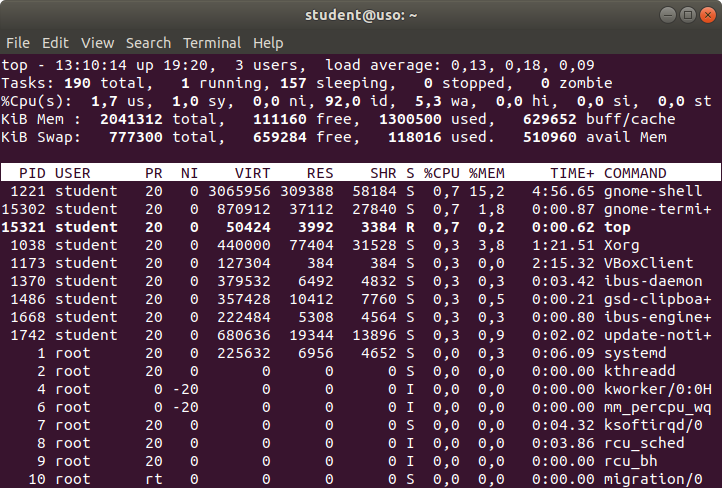
\includegraphics[width=0.8\textwidth]{chapters/04-process/img/top.png}
	\caption{Utilitarul top}
	\label{fig:process:top}
\end{figure}

\begin{figure}[!htbp]
	\centering
	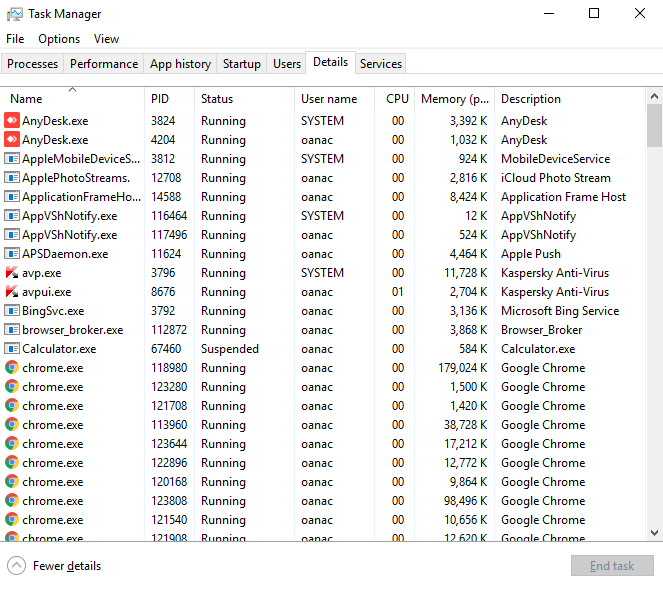
\includegraphics[width=0.8\textwidth]{chapters/04-process/img/task-manager.png}
	\caption{Utilitarul Task Manager}
	\label{fig:process:task-manager}
\end{figure}

Mai multe informații despre investigarea proceselor și monitorizarea resurselor
utilizate se găsesc în \labelindexref{Secțiunea}{sec:process:investigation}.

\subsection{Atributele unui proces}
\label{sec:process:attributes}

Un proces are atribute stabilite în mod normal la pornirea sa (la \textit{load-time}):
identificatorul procesului, procesul părinte, utilizatorul, prioritatea de
rulare. Unele atribuite sunt stabilite sau modificate la run-time. De exemplu,
prioritatea unui proces poate fi modificată pentru a afecta accesul la resurse;
un proces cu prioritate mai bună va avea acces mai des la procesor sau la disc
decât procese cu prioritate mai slabă.

Atributele unui proces au rolul de identifica un proces, de a stabili ce și cât
de multe resurse poate folosi și de a contabiliza resursele utilizate. O listă de
atribute de bază ale unui proces împreună cu o descriere a lor se găsește în
\labelindexref{Tabelul}{table:process:attributes}.

\begin{table}[!htb]
\caption{Atributele unui proces}
\begin{center}
  \begin{tabular}{ p{0.20\textwidth} p{0.40\textwidth} p{0.15\textwidth} p{0.10\textwidth}  }
	\toprule
                \textbf{atribut} & \textbf{rol} & \textbf{momentul atribuirii} & \textbf{modificabil} \\
	\midrule
                PID & identificare proces & pornire & nu \\
	\midrule
                PPID & identificare părinte proces & pornire & da \\
	\midrule
                program executabil & imaginea procesului (cod și date) & pornire & nu \\
	\midrule
                UID/GID (utilizator/grup) & permisiuni proces & pornire & nu (cu excepția unor situații punctuale) \\
	\midrule
                prioritate statică (\textit{nice}) & importanța în accesul resurselor & pornire & da \\
        \midrule
                terminal & interfața de comunicare cu utilizatorul & pornire & da \\
        \midrule
                fișiere deschise & lucrul cu fișiere & rulare & da \\
        \midrule
                stare & accesul curent la procesor & rulare & da \\
        \midrule
                timp de rulare pe procesor & contabilizare consum de procesor & rulare & da \\
        \midrule
                memorie consumată & contabilizare consum de memorie & rulare & da \\
        \midrule
                spațiu virtual de adrese & harta memoriei unui proces & pornire & da \\
	\bottomrule
	\end{tabular}
        \label{table:process:attributes}
\end{center}
\end{table}

Atributul PID este identificatorul unic al procesului la nivelul sistemului de
operare. Fiecare proces primește un identificator în momentul creării, atribut
ce nu se schimbă pe parcursul rulării. În general, comenzile sau funcțiile care
lucrează cu un proces primesc ca argument PID-ul acestui proces. De exemplu,
dacă vrem să terminăm un proces, vom folosi comanda \cmd{kill} cu argument PID-ul
acelui proces, ca în \labelindexref{Listing}{lst:process:kill-pid}.
În \labelindexref{Listing}{lst:process:kill-pid} se observă că există un proces generat din programul \cmd{sleep} cu PID-ul \texttt{9982}. Apoi procesul este omorât folosind comanda \cmd{kill} având ca argument PID-ul acelui proces.

\begin{screen}[caption={Terminarea unui proces folosind comanda kill},label={lst:process:kill-pid}]
student@uso:~$ ps -e | grep 9982
 9982 pts/2    00:00:00 sleep
student@uso:~$ kill 9982
student@uso:~$ ps -e | grep 9982
\end{screen}

Atributul UID \abbrev{UID}{User Id} este identificatorul utilizatorului ce
deține procesul. Un proces cu un anumit UID va avea acces la resursele acelui
utilizator. În mod normal, procesele aceluiași utilizator au acces la aceleași
resurse. Utilizatorii sunt modul principal de separare/izolare între procese.
Mai multe detalii vom prezenta în \labelindexref{Capitolul}{chapter:users}.

\subsection{Utilitare pentru urmărirea proceselor}
\label{sec:process:monitoring}

Sistemul de operare oferă utilitare și comenzi pentru a afișa
procese și pentru a urmări atributele și resursele lor.

Utilitarele din această categorie sunt de două tipuri:

\begin{itemize}
	\item cele care afișează un snapshot al momentului (procese active în
		acest moment și atribute ale lor)
	\item cele care monitorizează procesele sistemului
\end{itemize}

Din prima categorie fac parte, în Linux, utilitarele \cmd{ps}, \cmd{pgrep}, \cmd{pidof}, \cmd{pstree},
\cmd{pmap}, \cmd{lsof}. Din a doua categorie fac parte \cmd{top}, \cmd{htop}, \cmd{iotop}, \cmd{sysstat}. Pe Windows
utilitarele precum Task Manager, Process Explorer monitorizează procesele
sistemului.

Am prezentat în \labelindexref{Figura}{fig:process:top} și \labelindexref{Figura}{fig:process:task-manager} screenshot-uri cu utilitarele \cmd{top} și Task Manager, utilitare de monitorizare a proceselor. Monitorizarea
proceselor e utilă pentru a urmări procesele din sistem, a observa tendințe, a
vedea consumul de resurse și pentru a investiga de ce sistemul sau un proces
funcționează anevoios. Mai multe informații despre monitorizarea și investigarea
proceselor vom prezenta în \labelindexref{Secțiunea}{sec:process:investigation}.

Mai jos sunt descrise utilitarele pentru afișarea de informații de tip snapshot
despre procese:

\begin{itemize}
  \item \cmd{ps} este principalul utilitar de afișare de informații despre
		procese. La o rulare simplă afișează procesele din terminalul
		curent. Poate afișa selectiv procese și atribute ale acestora.
  \item \cmd{pidof} afișează PID-ul proceselor care au un anumit program
		(imagine de proces)
  \item \cmd{pgrep} are funcționalitatea utilitarului \cmd{pidof} extinsă: afișează procesele
		care corespund unei anumite condiții. Condiția poate fi
		,,aparține unui anumit utilizator'', ,,are un anumit program ca
		imagine'', ,,are un anumit proces părinte'', ,,rulează într-un
		anumit terminal'', la fel ca în exemplele de mai jos.
  \item \cmd{pstree} afișează ierarhia de procese a sistemului, îl vom detalia
    în \labelindexref{Secțiunea}{sec:process:linux-hierarchy}.
  \item \cmd{pmap} (\textit{process map}) afișează harta memoriei unui proces,
		adică zonele de memorie ocupate de acesta. Este un utilitar
		adecvat în special pentru programatori și pentru cei care sunt
		interesați de internele sistemelor de operare, nu insistăm pe
		el.
  \item \cmd{lsof} (\textit{list open files}) este utilitarul care afișează
		fișierele deschise de un proces. Îl vom folosi în
		\labelindexref{Secțiunea}{sec:process:files}
\end{itemize}

Așa cum am precizat, utilitarul \cmd{ps} este utilitarul principal pentru listarea
proceselor și a atributelor acestora. Am prezentat exemple de investigare a proceselor folosind utilitarul \cmd{ps} în \labelindexref{Listing}{lst:process:ps}. \labelindexref{Listing}{lst:process:ps-extra} conține scenarii frecvente de folosire a comenzii \cmd{ps} cu argumentele aferente. Comenzile rulate în \labelindexref{Listing}{lst:process:ps-extra} au următorul efect:
\begin{itemize}
	\item linia 1: listarea tuturor proceselor din sistem
	\item linia 8: listarea tuturor proceselor fără afișarea capului de tabel
	\item linia 15: listarea cu mai multe atribute a proceselor din sistem
        \item linia 22: listarea proceselor ce aparțin utilizatorului \texttt{student}
        \item linia 29: listarea proceselor ce nu aparțin utilizatorului \texttt{student}
        \item linia 36: listarea proceselor ce au imagine (program) \cmd{VBoxClient}
	\item linia 43: listarea doar a PID-urilor, comenzii de pornire, procentul de
		procesor acaparat și memorie utilizate pentru toate procesele
	\item linia 50: listarea doar a PID-urilor, comenzii de pornire și a stării pentru
          procesele ce aparțin utilizatorului \texttt{student}
	\item linia 57: listarea doar a PID-urilor, comenzii de pornire, procentul de
		procesor acaparat și memorie utilizate pentru toate procesele
                sortate după procentul de procesor acaparat pentru procesele ce aparțin utilizatorului \texttt{student}
\end{itemize}

\begin{screen}[caption={Folosirea comenzii ps},label={lst:process:ps-extra}]
student@uso:~$ ps -e
  PID TTY          TIME CMD
    1 ?        00:00:05 systemd
    2 ?        00:00:00 kthreadd
    4 ?        00:00:00 kworker/0:0H
    6 ?        00:00:00 mm_percpu_wq
[...]
student@uso:~$ ps -e --no-header
    1 ?        00:00:05 systemd
    2 ?        00:00:00 kthreadd
    4 ?        00:00:00 kworker/0:0H
    6 ?        00:00:00 mm_percpu_wq
    7 ?        00:00:03 ksoftirqd/0
[...]
student@uso:~$ ps -e -f
UID        PID  PPID  C STIME TTY          TIME CMD
root         1     0  0 01:04 ?        00:00:05 /sbin/init splash
root         2     0  0 01:04 ?        00:00:00 [kthreadd]
root         4     2  0 01:04 ?        00:00:00 [kworker/0:0H]
root         6     2  0 01:04 ?        00:00:00 [mm_percpu_wq]
[...]
student@uso:~$ ps -u student
  PID TTY          TIME CMD
 1018 ?        00:00:01 systemd
 1019 ?        00:00:00 (sd-pam)
 1032 ?        00:00:00 gnome-keyring-d
 1036 tty1     00:00:00 gdm-x-session
[...]
student@uso:~$ ps -N -u student
  PID TTY          TIME CMD
    1 ?        00:00:05 systemd
    2 ?        00:00:00 kthreadd
    4 ?        00:00:00 kworker/0:0H
    6 ?        00:00:00 mm_percpu_wq
[...]
student@uso:~$ ps -C VBoxClient
  PID TTY          TIME CMD
 1148 ?        00:00:00 VBoxClient
 1149 ?        00:00:00 VBoxClient
 1159 ?        00:00:00 VBoxClient
 1160 ?        00:00:00 VBoxClient
[...]
student@uso:~$ ps -e -o pid,cmd,%cpu,rss
  PID CMD                         %CPU   RSS
    1 /sbin/init splash            0.0  7292
    2 [kthreadd]                   0.0     0
    4 [kworker/0:0H]               0.0     0
    6 [mm_percpu_wq]               0.0     0
[...]
student@uso:~$ ps -u student -o pid,cmd,%cpu,rss
  PID CMD                         %CPU   RSS
 1018 /lib/systemd/systemd --user  0.0  5552
 1019 (sd-pam)                     0.0   260
 1032 /usr/bin/gnome-keyring-daem  0.0  4608
 1036 /usr/lib/gdm3/gdm-x-session  0.0  3928
[...]
student@uso:~$ ps -u student -o pid,cmd,%cpu,rss --sort -%cpu
  PID CMD                         %CPU   RSS
 1221 /usr/bin/gnome-shell         0.4 292668
 8637 /usr/bin/python3 /usr/bin/u  0.4 80232
 2637 /usr/lib/firefox/firefox -n  0.2 264472
 2717 /usr/lib/firefox/firefox -c  0.2 115660
[...]
\end{screen}

Dacă la un moment dat avem nevoie de PID-urile proceselor care au un anumit program ca imagine, vom folosi comanda:

\begin{screen}
student@uso:~$ ps -o pid -C VBoxClient
  PID
 1148
 1149
 1159
 1160
[...]
\end{screen}

La fel, dacă avem nevoie de PID-urile proceselor unui anumit utilizator, vom
folosi comanda:

\begin{screen}
student@uso:~$ ps -o pid -u student
  PID
 1018
 1019
 1032
 1036
[...]
\end{screen}

Observăm că avem inclusiv antetul afișării, deși ne dorim doar PID-urile. Pentru
aceasta, folosim caracterul \texttt{=} după numele argumentului \texttt{pid}, în forma \texttt{pid=} care
dezactivează afișarea header-ului:

\begin{screen}
student@uso:~$ ps -o pid= -C VBoxClient
 1148
 1149
 1159
 1160
[...]
student@uso:~$ ps -o pid= -u student
 1018
 1019
 1032
 1036
[...]
\end{screen}

De avut în vedere că același lucru poate fi obținut, mai simplu, folosind
comanda \cmd{pgrep}:

\begin{screen}
student@uso:~$ pgrep VBoxClient
1148
1149
1159
1160
[...]
student@uso:~$ pgrep -u student
1018
1019
1032
1036
[...]
\end{screen}

Atunci când dorim să obținem doar PID-urile anumitor procese, este mai simplu să
folosim \cmd{pgrep} în loc de \cmd{ps}.

\subsection{Starea proceselor}
\label{sec:process:state}

Într-unul din exemplele de folosire a utilitarului \cmd{ps} de mai sus am vorbit
despre starea unui proces. Un proces are o stare care arată dacă acesta rulează
sau nu pe procesor.

Un proces are nevoie de unul sau mai multe procesoare pentru a rula. Întrucât,
de cele mai multe ori, sunt mai multe procese decât procesoare, nu toate
procesele pot rula. Astfel unele procese rulează pe procesor, altele așteaptă să
ruleze pe procesor; când un proces ajunge să ruleze pe un procesor spunem că
este planificat (\textit{scheduled}) să ruleze pa acel procesor. Iar unele
procese pot fi blocate (\textit{sleeping}) în așteptarea unei operații de
input/output. Simplificat, avem precizate stările și tranzițiile între stările unui proces în \labelindexref{Figura}{fig:process:state}.

\begin{figure}[!htbp]
	\centering
	\def\svgwidth{0.8\textwidth}
	\includesvg{chapters/04-process/img/proc-status.svg}
	\caption{Starea proceselor}
	\label{fig:process:state}
\end{figure}

Putem investiga starea proceselor cu utilitare de urmărire și monitorizare.
Acest lucru este util pentru a vedea dacă un proces este blocat și pentru ca
apoi să investigam cauza pentru care este blocat. Sau să vedem cât de multe
procese sunt active, gata să ruleze. În \labelindexref{Listing}{lst:process:ps-monitor} am afișat PID-ul,
imaginea, starea, timpul de rulare și procentul curent de procesor ocupat pentru
toate procesele din sistem, sortate în ordinea inversă a procentului de procesor ocupat. În rezultatul comenzii \cmd{ps}, \texttt{R} înseamnă \textit{runnable} (nu \textit{running}), adică fie rulează
atunci pe procesor (starea \textit{running}) fie poate fi pregătit să ruleze (starea
\textit{ready}).

\begin{screen}[caption={Monitorizarea proceselor folosind ps},label={lst:process:ps-monitor}]
student@uso:~$ ps -e -o pid,cmd,state,time,%cpu --sort -%cpu
  PID CMD                         S     TIME %CPU
 8637 /usr/bin/python3 /usr/bin/u S 00:00:22  3.6
 9042 /usr/lib/snapd/snapd        S 00:00:05  1.2
 1221 /usr/bin/gnome-shell        S 00:04:03  0.4
 2717 /usr/lib/firefox/firefox -c S 00:02:05  0.3
 2637 /usr/lib/firefox/firefox -n S 00:02:01  0.2
\end{screen}

Un sistem este cu atât mai încărcat cu cât are mai multe procese gata să ruleze,
dar care nu au fost planificate. Aceste procese se cheamă \textit{ready} sau \textit{runnable} așa
cum sunt prezente în \labelindexref{Figura}{fig:process:state}. Când multe procese sunt \textit{ready} înseamnă
că vor acapara un procesor imediat ce acesta devine disponibil și vor ține
procesorul și sistemul încărcat.

Noțiunea de încărcare a unui sistem (numită și \textit{load}) este dată de numărul de
procese \textit{ready}. Utilitarul \cmd{uptime} ne afișează încărcarea unui sistem în ultimul
minut, în ultimele 5 minute și în ultimele 15 minute, ca în exemplul de mai jos:

\begin{screen}
student@uso:~$ uptime
13:48:40  up 9 days 16:13,  5 users,  load average: 1.61, 2.05, 2.81
\end{screen}

Încărcarea unui sistem (\textit{load average}) este deci \texttt{1.61} (în ultimul minut), \texttt{2.05} (în ultimele 5 minute), \texttt{2.81} în ultimele 15 minute. Valoarea încărcării este corelată cu numărul de procese în starea \textit{ready}: pregătite de execuție dar care încă nu pot rula pentru că procesoarele sistemului sunt ocupate.

Utilitarul \cmd{top} afișează, în partea superioară, informații despre încărcarea
sistemului:

\begin{screen}
top - 13:58:20 up 14:02,  2 users,  load average: 0,71, 1,31, 0,92
Tasks: 190 total,   1 running, 156 sleeping,   0 stopped,   0 zombie
%Cpu(s):  1,3 us,  0,3 sy,  0,2 ni, 97,9 id,  0,3 wa,  0,0 hi,  0,0 si,  0,0 st
KiB Mem :  2041312 total,    70676 free,  1287316 used,   683320 buff/cache
KiB Swap:   777300 total,   699476 free,    77824 used.   531880 avail Mem
\end{screen}

\subsection{Prioritatea proceselor}
\label{sec:process:priority}

Procesele concurează la folosirea procesorului. Sistemul de operare planifică un
proces \textit{ready} pe procesor ținând cont de prioritatea sa. Procesele cu prioritate
mai bună sunt planificate mai des și rulează mai mult timp pe procesor.
Prioritatea unui proces este afectată de comportamentul acestuia (procesele mai
,,flămânde'' primesc o prioritate mai slabă) și poate fi afectată de utilizator.

În Windows, utilizatorul poate afecta prioritatea unui proces folosind Task Manager, așa cum apare în \labelindexref{Figura}{fig:process:priority-task-manager}.

\begin{figure}[!htbp]
	\centering
	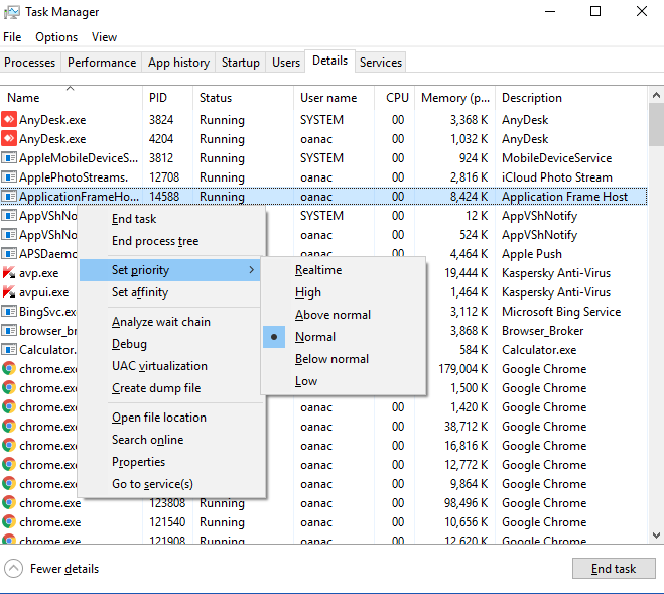
\includegraphics[width=0.8\textwidth]{chapters/04-process/img/task-manager-priority.png}
	\caption{Priorități de procese în Windows}
	\label{fig:process:priority-task-manager}
\end{figure}

În Linux, putem modifica prioritatea unui proces prin schimbarea atributului \texttt{nice} al procesului.
Valoarea \texttt{nice} arată cât de ,,drăguț'' este acel proces cu alte
procese. O valoare mai mare a \texttt{nice} înseamnă că procesul este mai drăguț, deci
lasă alte procese să fie planificate; o valoare mai mică a \texttt{nice} înseamnă că
procesul nu este drăguț, deci ,,va lua fața'' altor procese. Aceste lucru înseamnă
că o valore \texttt{nice} mică înseamnă un proces cu prioritate mai bună, iar o valoare
\texttt{nice} mare înseamnă un proces cu prioritate mai slabă.

\begin{note}[Exprimări legate de prioritatea proceselor]
Din cauză că există această inconsecvență între valoarea \texttt{nice} și prioritate
folosim exprimarea ,,prioritate mai bună'' și ,,prioritate mai slabă''.
Folosirea exprimării ,,prioritate mai mare'' și ,,prioritate mai mică'' ar
putea produce confuzie între prioritate și valoarea \texttt{nice}.
\end{note}

În mod implicit un proces pornește cu valoarea \texttt{nice} 0, o valoare neutră.
Valoarea poate fi modificatăla pornirea procesului (\textit{load-time}) sau în timp ce
rulează (\textit{run-time}). Un utilizator obișnuit (neprivilegiat) poate doar crește
valoarea \texttt{nice} a unui proces pe care îl deține, adică în sensul slăbirii
priorității procesului. Doar un utilizator privilegiat poate scădea valoarea
\texttt{nice} a unui proces, adică în sensul îmbunătățirii priorității procesului.

Pentru a modifica prioritatea unui proces la pornire (\textit{load-time}) folosim
utilitarul \cmd{nice}. Pentru a modifica prioritatea unui proces la rulare (\textit{run-time})
folosim utilitarul \cmd{renice}. \labelindexref{Listing}{lst:process:nice} conține exemple de comenzi care
modifică prioritatea unui proces; după fiecare comandă \cmd{nice} / \cmd{renice} folosim \cmd{ps}
pentru a vedea acum noua prioritate a procesului.

În \labelindexref{Listing}{lst:process:nice} am folosit comanda \cmd{renice} pentru a modifica valoarea \texttt{nice} a unui proces. Comanda poate fi folosită de un utilizator neprivilegiat doar pentru a crește, nu și pentru a scădea valoarea \texttt{nice} a unui proces. Pentru scădea valoarea \texttt{nice} a unui proces folosim contul privilegiat, cu ajutorul comenzii \cmd{sudo}. Similar, comanda \cmd{nice} poate porni un proces cu valoarea \texttt{nice} modificată.

\begin{screen}[caption={Modificarea priorității unui process (nice)},label={lst:process:nice}]
student@uso:~$ sleep 1000 &
[1] 10384
student@uso:~$ ps -C sleep -o pid,uid,nice,cmd
  PID   UID  NI CMD
10384  1000   0 sleep 1000
student@uso:~$ renice +10 10384
10384 (process ID) old priority 0, new priority 10
student@uso:~$ ps -C sleep -o pid,uid,nice,cmd
  PID   UID  NI CMD
10384  1000  10 sleep 1000
student@uso:~$ renice +0 10384
renice: failed to set priority for 10384 (process ID): Permission denied

student@uso:~$ sudo renice -20 10384
10384 (process ID) old priority 0, new priority -20
student@uso:~$ ps -C sleep -o pid,uid,nice,cmd
  PID   UID  NI CMD
10384  1000 -20 sleep 1000

student@uso:~$ nice -n +10 sleep 1000 &
[1] 10410
student@uso:~$ ps -C sleep -o pid,uid,nice,cmd
  PID   UID  NI CMD
10410  1000  10 sleep 1000

student@uso:~$ nice -n -10 sleep 1000 &
[1] 10412
student@uso:~$ nice: cannot set niceness: Permission denied

student@uso:~$ sudo nice -n -10 sleep 1000 &
[1] 10413
student@uso:~$ ps -C sleep -o pid,uid,nice,cmd
  PID   UID  NI CMD
10414     0 -10 sleep 1000
\end{screen}

Prioritatea unui proces este principalul mijloc prin care un proces poate folosi
mai mult sau mai puțin procesorul unui sistem. Dacă vrem ca un proces să
folosească mai mult resursele sistemului, vom îmbunătăți prioritatea acestuia;
dacă un proces utilizează prea mult resursele sistemului (\textit{resource hog}) și vrem să-l
,,temperăm'', îi slăbim prioritatea; la nevoie un astfel de proces este omorât.

\section{Ierarhia de procese}
\label{sec:process:hierarhy}

Un proces este creat la comanda utilizatorului sau la un eveniment de declanșare
(o nouă conexiune în rețea, expirarea unui interval de timp). Așa cum am precizat un proces este creat la \textbf{load-time}
dintr-un fișier executabil (numit imagine de proces); după creare
procesului îi sunt alocate resurse (precum timp de procesor și zone de memorie)
și rulează (\textbf{run-time}).

\begin{definition}{Loading}
Crearea unui proces dintr-un executabil se mai numește
\textit{loading} (încărcare executabilului în memorie), iar momentul creării se numește \textbf{load-time}.
\end{definition}

Un proces este creat prin intermediul unui alt proces, numit \textbf{proces părinte} (\textit{parent process}). Un
proces poate crea oricâte \textbf{procese copil} (\textit{child process}), în limita resurselor sistemului. Un
proces poate avea, însă, un singur proces părinte. Pentru crearea unui proces,
procesul părinte folosește o interfață specifică a sistemului de operare:
folosește grupul de apeluri \texttt{fork()} și \texttt{exec()} în Linux și \texttt{CreateProcess()} pe
Windows. Nu insistăm pe aceste apeluri în această carte; câteva detalii găsiți
în \labelindexref{Secțiunea}{sec:cli-new-process}. Vizual,
crearea unui proces este indicată în \labelindexref{Figura}{fig:process:create}.

\begin{figure}[!htbp]
	\centering
	\def\svgwidth{0.5\textwidth}
	\includesvg{chapters/04-process/img/fork-exec.svg}
	\caption{Crearea unui proces}
	\label{fig:process:create}
\end{figure}

În general, procesul care creează un nou process este un shell. Shellul poate
fi grafic (precum \textbf{Windows Explorer}) sau poate fi în linia de comandă (precum
\textbf{Bash}). De exemplu, în mediul grafic, atunci când folosim dublu click pe o icoană
de pe ecran, pornim un proces; acel proces este creat de shellul grafic, care
define procesul părinte al noului proces. Altfel, în linia de comandă, shellul
creează un proces nou la introducerea unei comenzi. Prezentăm mai multe detalii
în \labelindexref{Capitolul}{chapter:cli}.

Legătura proces părinte - proces copil este utilă pentru a afla informații legate
de încheierea unui proces. Un proces își poate încheia execuția în mai multe
moduri: ajunge la sfârșitul zonei de execuție, este omorât de alt proces,
execută o acțiune nevalidă. Procesul părinte este cel care poate furniza
informații despre condițiile de încheiere ale unui proces copil.

\subsection{Ierarhia de procese în Linux/Unix}
\label{sec:process:linux-hierarchy}

În Linux, întrucât un proces creează alt proces care la rândul său poate crea
alt proces, procesele sunt organizate într-o ierarhie de procese, într-o
aborescență. De exemplu la o rulare a comenzii \cmd{pstree} putem vedea ierarhia de
procese în Linux ca în \labelindexref{Listing}{lst:process:pstree}.
Cu opțiunea \texttt{-p}, comanda \cmd{pstree} afișează și PID-ul proceselor.

\begin{screen}[caption={Ierarhia de procese în Linux},label={lst:process:pstree}]
student@uso:~$ pstree -A
systemd-+-ModemManager---2*[{ModemManager}]
        |-NetworkManager-+-2*[dhclient]
        |                `-2*[{NetworkManager}]
        |-2*[VBoxClient---VBoxClient---{VBoxClient}]
        |-VBoxClient---VBoxClient
        |-VBoxClient---VBoxClient---2*[{VBoxClient}]
        |-VBoxService---7*[{VBoxService}]
        |-accounts-daemon---2*[{accounts-daemon}]
[...]
student@uso:~$ pstree -A -p
systemd(1)-+-ModemManager(447)-+-{ModemManager}(466)
           |                   `-{ModemManager}(475)
           |-NetworkManager(473)-+-dhclient(9735)
           |                     |-dhclient(9769)
           |                     |-{NetworkManager}(573)
           |                     `-{NetworkManager}(581)
           |-VBoxClient(1148)---VBoxClient(1149)---{VBoxClient}(1155)
           |-VBoxClient(1159)---VBoxClient(1160)
           |-VBoxClient(1166)---VBoxClient(1167)---{VBoxClient}(1168)
           |-VBoxClient(1172)---VBoxClient(1173)-+-{VBoxClient}(1174)
           |                                     `-{VBoxClient}(1175)
[...]
\end{screen}

Observăm că în vârful ierarhiei, în rădăcina proceselor, se găsește procesul \textbf{systemd},
procesul cu PID-ul 1. \textbf{systemd} este o implementare de proces \textbf{init}. În mod generic, spunem că primul proces al sistemului, rădăcina ierarhiei de procese, este \textbf{init}, cu diferite forme de implementare. Implementarea folosită curent în majoritatea distribuțiilor Linux este \textbf{systemd}.

\textbf{init} este primul proces al sistemului, procesul care
pornește serviciile sistemului și procesele de bază. În \labelindexref{Listing}{lst:process:pstree} observăm că un
proces are un singur proces părinte și oricâte procese copil. Ierarhia nu are
foarte multe niveluri. În general procesul init creează servicii de bază și
shelluri, iar shellurile creează alte procese. Detalii despre procesul init
prezentăm în \labelindexref{Secțiunea}{sec:process:init}

În mod obișnuit, un proces dat are, de la creare până la încheiere, un proces
părinte. Se poate întâmpla însă ca un proces să rămână ,,orfan'' adică procesul
părinte să își încheie execuția înaintea sa. În acest caz, în Linux, procesul
init ,,adoptă'' procesul rămas orfan și devine noul proces părinte. Vom prezenta
detalii în \labelindexref{Secțiunea}{sec:process:init}.

\subsection{Ierarhia de procese în Windows}
\label{sec:process:windows-hierarchy}

În Windows, în mod similar, un proces creează alt proces. Cu toate acestea
ierarhia de procese în Windows este o ierarhie cu legături mai slabe. În vreme
ce în Linux, un proces părinte are privilegii specifice de comunicare cu un
proces copil (de exemplu comunicare prin operatorul \textit{pipe}), în Windows un proces poate comunica în
același mod cu un proces părinte și cu un proces cu care nu este conectat
ierarhic. Un proces are o referință (\textit{handle}) către un proces pe care l-a creat, dar acea referință poate fi transferată altui proces, afectând ierarhia. Mai mult, în Windows orice proces poate obține informații despre
încheierea unui alt proces, spre deosebire de Linux unde doar procesul părinte
poate obține informații.

O imagine a ierarhiei de procese în Windows putem obține folosind utilitarul
Process Explorer, așa cum vedem în \labelindexref{Figura}{fig:process:process-explorer-hierarchy}

\begin{figure}[!htbp]
	\centering
	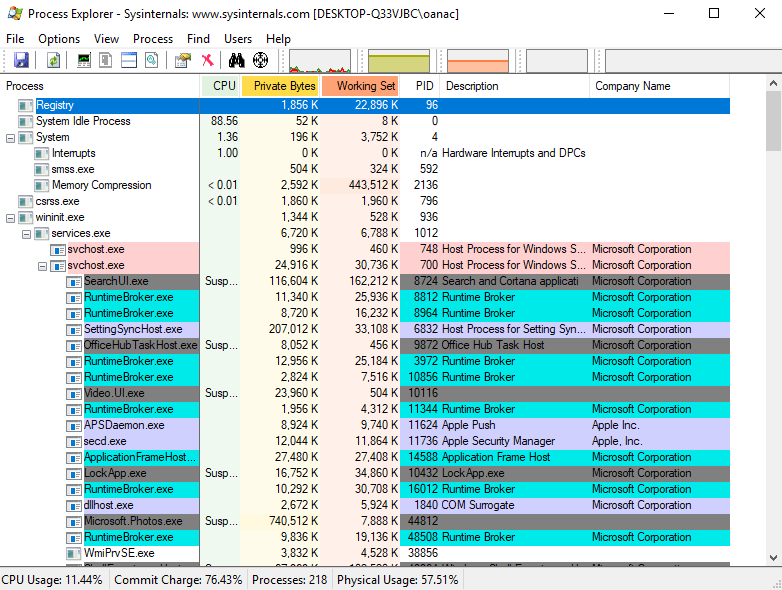
\includegraphics[width=0.8\textwidth]{chapters/04-process/img/process-explorer.png}
	\caption{Vizualizare ierarhie de procese folosind Process Explorer}
	\label{fig:process:process-explorer-hierarchy}
\end{figure}

Shellul Windows este un shell grafic reprezentat de procesul Explorer, prezent în \labelindexref{Figura}{fig:process:process-explorer-hierarchy}. Acest
proces creează aplicațiile/procesele pornite în mediul grafic în Windows.

\subsection{Foreground și background}
\label{sec:process:foreground-background}

Un proces shell în linia de comandă creează procese în momentul introducerii de
comenzi din partea utilizatorului. Procesul nou creat și shellul folosesc
simultan terminalul, adică modul în care utilizatorul poate transmite informații
la ieșirea standard și modul în care se afișează mesaje la ieșirea standard.
Dacă atât procesul nou creat cât și shellul afișează informații la ieșirea
standard, aceste afirmații vor fi agregate și afișate la terminal. Dacă însă
trimitem informații la intrarea standard, prin terminal, doar procesul nou creat
la va accesa.

Spunem că, în cadrul terminalului, avem un singur proces care deține controlul
intrării standard, adică un singur proces care este în \textbf{foreground}. În
general, modul de funcționare a shellului, detaliat în \labelindexref{Secțiunea}{sec:cli-shell-func}, este:

\begin{enumerate}
	\item shellul citește de la intrarea standard (din terminal) comenzi și
		opțiuni ale utilizatorului
	\item shellul creează un nou proces pornind de la comanda introdusă
        \item procesul nou creat rulează în \textbf{foreground} și are controlul
		terminalului (și a intrării acestuia)
	\item procesul nou creat își încheie execuția; shellul, în calitate de
		proces părinte, reține informații despre încheierea execuției
	\item shellul redobândește controlul terminalului și reîncepem acțiunea
		de la punctul 1
\end{enumerate}

Acest mod de funcționare devine problematic în momentul în care procesul nou
creat nu își încheie rapid execuția: fie rulează mai mult, fie este o aplicație
grafică folosită interactiv de utilizartor. În această situație, procesul nou
creat ,,acaparează'' terminalul și împiedică shellul să citească noi comenzi și
să creeze noi proces. De exemplu dacă introducem comanda \cmd{firefox}, shellul va
crea un proces Firefox care va acapara terminalul.

Pentru a trece de această problemă și pentru a permite shellului rularea
continuă de comenzi și crearea de mai multe procese, există un mod de folosire a
terminalului numit \textbf{background}. Background este modul în care un proces
cedează accesul la intrarea terminalului curent; procesul poate rula în
continuare dar nu mai are acces la informații furnizate de utilizator.

Întrucât un singur proces poate avea acces la intrarea terminalului, putem avea
un singur proces în foreground. Putem avea însă oricâte procese în background.
În background proceswle se pot găsi în două stări: rulând (\textit{running}) sau
suspendate (\textit{stopped}, \textit{suspeneded}, \textit{paused}). Decizia de a suspenda și de a scoate
un proces din starea suspendat aparține utilzatorului. Un proces suspendat nu se
poate găsi în foreground, ci doar în background.

Un proces poate rula de la început în background sau poate fi transferat în
background după pornire. De exemplu, pentru a rula un proces în background
folosim operatorul \texttt{\&} imediat după comanda aferentă și parametrii acesteia. În \labelindexref{Listing}{lst:process:background-start},
în prima rulare a comenzii, procesul Firefox a fost pornit în foreground,
iar apoi, folosind operatorul \texttt{\&}, procesul Firefox a fost pornit în background.
Comanda \cmd{jobs} este folosită pentru a afișa job-urile din shellul curent, adică
procesele care se găsesc în background.

\begin{screen}[caption={Pornirea unui process în background},label={lst:process:background-start}]
student@uso:~$ firefox
student@uso:~$ firefox &
[1] 10533
student@uso:~$ jobs
[1]+  Running                 firefox &
\end{screen}

În cazul rulării unei comenzi în mod simplu, fără operatorul \texttt{\&}, procesul
pornește în foreground. Poate fi adus ulterior în background folosind combinația
de taste \texttt{Ctrl+z}. Această combinație de taste are ca efect suspendarea
procesului. Întrucât procesul nu poate rula suspendat în foreground, este trecut
în background, ca în \labelindexref{Listing}{lst:process:background-suspend}.

\begin{screen}[caption={Suspendarea unui process în background},escapechar=,label={lst:process:background-suspend}]
student@uso:~$ sleep 100
^Z
[1]+  Stopped                 sleep 100
student@uso:~$ jobs
[1]+  Stopped                 sleep 100
\end{screen}

Observăm așadar că folosirea operatorului \texttt{\&} duce un proces în background în
starea rulând, pe când folosirea combinației de taste \texttt{Ctrl+z} duce un proces în
background în starea suspendat. O dată dus un proces în background acesta poate
fi readus în foreground folosind comanda \cmd{fg}, ca în \labelindexref{Listing}{lst:process:fg}.
În \labelindexref{Listing}{lst:process:fg} rulăm o comandă obișnuit și procesul rezultat rulează în
background. Ulterior, folosim \texttt{Ctrl+z} pentru a plasa procesul în background. Apoi
folosim \cmd{fg} pentru a-l readuce în foreground. În momentul în care este în background, procesul apare ca job, afișat în rezultatul rulării comenzii \cmd{jobs}. Când un proces este în background, acesta acaparează terminalul; în acest caz, alte informații trimise la intrare (precum introducerea comanda \cmd{ls}) nu sunt interpretate de shell.

\begin{screen}[caption={Readucerea unui process în foreground},escapechar=,label={lst:process:fg}]
student@uso:~$ sleep 100
^Z
[1]+  Stopped                 sleep 100
student@uso:~$ jobs
[1]+  Stopped                 sleep 100
student@uso:~$ fg
sleep 100
ls
^C
student@uso:~$ jobs
student@uso:~$
\end{screen}

Un proces dus în background în starea suspendat folosind combinația de taste
\texttt{Ctrl+z} poate fi apoi trecut în starea \textit{running}, tot în background. Facem acest
lucru folosind comanda \cmd{bg}, ca în \labelindexref{Listing}{lst:process:bg}.
În \labelindexref{Listing}{lst:process:bg} se observă că, după folosirea combinației de taste \texttt{Ctrl+z}, procesul ajunge în starea \texttt{Stopped} în background. Apoi, prin folosirea comenzii \texttt{bg} acesta ajunge în starea \texttt{Running} în background.

\begin{screen}[caption={Trecerea unui proces în starea running în background},escapechar=,label={lst:process:bg}]
student@uso:~$ sleep 100
^Z
[1]+  Stopped                 sleep 100
student@uso:~$ jobs
[1]+  Stopped                 sleep 100
student@uso:~$ bg
[1]+ sleep 100 &
student@uso:~$ jobs
[1]+  Running                 sleep 100 &
\end{screen}

Sumarizând, \labelindexref{Figura}{fig:process:fg-bg} prezintă modul în care poate rula un proces în
background/foreground: ce comenzi și operatori sunt folosiți în fiecare caz, ce
stări au procesele și cum pot tranzita între stări (\textit{running}, \textit{stopped}) și între
moduri de rulare (foreground, background).

\begin{figure}[!htbp]
	\centering
	\def\svgwidth{0.8\textwidth}
	\includesvg{chapters/04-process/img/status-mov.svg}
	\caption{Foreground și background}
	\label{fig:process:fg-bg}
\end{figure}

Am precizat că mai multe procese pot rula în background. Procesele care rulează
în background se numesc joburi și au un identificator de job pentru shellul
curent. Dacă avem mai multe joburi dorim să controlăm starea unui job folosind
comenzile \cmd{fg} și \cmd{bg}, atunci vom adăuga ca parametru către aceste comenzi
identificatorul jobului, așa cum facem în \labelindexref{Listing}{lst:process:job-id}.
În \labelindexref{Listing}{lst:process:job-id} am folosit construcțiile \texttt{\%1} și \texttt{\%2} pentru a opera joburile cu indexul 1 și 2 din background. Am trimis indexul ca argument comenzilor \cmd{bg} și \cmd{fg}.

\begin{screen}[caption={Gestiunea job-urilor},label={lst:process:job-id}]
student@uso:~$ sleep 100 &
[1] 10962
student@uso:~$ sleep 200
^\verb+^+^Z
[2]+  Stopped                 sleep 200
student@uso:~$ jobs
[1]-  Running                 sleep 100 &
[2]+  Stopped                 sleep 200
student@uso:~$ bg %2
[2]+ sleep 200 &
student@uso:~$ jobs
[1]-  Running                 sleep 100 &
[2]+  Running                 sleep 200 &
student@uso:~$ fg %2
sleep 200
^\verb+^+^Z
[2]+  Stopped                 sleep 200
student@uso:~$ jobs
[1]-  Running                 sleep 100 &
[2]+  Stopped                 sleep 200
student@uso:~$ fg %1
sleep 100
^\verb+^+^C
student@uso:~$ jobs
[2]+  Stopped                 sleep 200
\end{screen}

Un scenariu util pentru trecerea unui proces în background este când pornim un
proces GUI \abbrev{GUI}{Graphical User Interface} din shell și pierdem în shell
accesul la terminal. De exemplu am pornit procesul Emacs (grafic) în foreground.
Pentru a putea readuce shellului controlul terminalului, vom trece procesul
Emacs în background (suspendat) folosind combinația de taste \texttt{Ctrl+z} și vom muta
apoi procesul din starea supendat în starea running folosind comanda bg. Adică
la fel în \labelindexref{Listing}{lst:process:background-gui}.

\begin{screen}[caption={Transferul unui proces GUI din foreground în background},label={lst:process:background-gui}]
student@uso:~$ emacs
^\verb+^+^Z
[1]+  Stopped                 emacs
student@uso:~$ bg
[1]+ emacs &
student@uso:~$ jobs
[1]+  Running                 emacs &
\end{screen}

În mod obișnuit, dacă un shell se închide (se rulează comanda \cmd{exit} sau
combinația \texttt{Ctrl+d} sau este închisă fereastra terminalului în care rulează),
procesele active în terminalul respectiv sunt, de asemenea, omorâte. Sunt
omorâte procesele aflate în background și, eventual, procesul aflat în
foreground. Dacă dorim să menținem anumite procese active după încheierea
procesului shell, avem opțiuni de lucru; vom discuta despre aceste opțiuni în
\labelindexref{Secțiunea}{sec:process:daemon}.

\subsection{Procesul init}
\label{sec:process:init}

După cum am indicat în \labelindexref{Secțiunea}{sec:process:linux-hierarchy},
în vârful ierarhiei proceselor din Linux se găsește procesul \textbf{init}. Acesta este
primul proces al sistemului și creatorul primelor procese. Serviciile de bază
ale sistemului, shellurile inițiale, mediul grafic sunt pornite direct sau
indirect din procesul init. Spunem că un sistem Linux a bootat în momentul
creării procesului init. În această secțiune discutăm minimal despre init, cu
accent pe rolul său în gestiunea proceselor sistemului. Detalii despre pornirea
sistemului până la pornirea init, și detalii despre init și configurarea sa
prezentăm în \labelindexref{Capitolul}{chapter:boot}.

Pe lângă rolul în pornirea proceselor inițiale, init are și rol în întreținerea
sistemului prin adoptarea proceselor orfane. Un proces orfan este un proces al
cărui proces părinte și-a încheiat execuția. Pentru a menține ierarhia de
procese, acest proces trebuie să aibă un proces părinte; acest proces părinte
este procesul init. În codul sursă de suport al cărții în directorul \file{code/04-process/code/parent-child/} este un exemplu în care creăm un proces părinte (implementat fișierul sursă C \file{parent.c}) care apoi creează un proces (implementat în fișierul sursă C \file{child.c}). \labelindexref{Listing}{lst:process:init-adopt} conține o secvență în care rulăm programul ce creează procesul părinte, program care apoi creează procesul copil.
În \labelindexref{Listing}{lst:process:init-adopt} în prima parte am pornit procesul \texttt{parent} care apoi a pornit și procesul \texttt{child}. Apoi din alt terminal urmărim cele două procese și observăm că procesul copil (\texttt{child}) cu PID-ul \texttt{11305} are ca părinte procesul părinte (\texttt{parent}) cu PID-ul \texttt{11304}. Apoi omorâm procesul părinte și investigăm din nou procesul copil. Observăm că acum procesul părinte este procesul \texttt{init} cu PID-ul \texttt{1}.

\begin{screen}[caption={Adoptarea unui proces orfan de către proces init},label={lst:process:init-adopt}]
# start process
student@uso:~/.../code/04-process/parent-child$ ./parent
parent: Parent process started. Creating child process ...
parent: Child process created. Now going to sleep ...
child: Child process started. Now going to sleep ...

# investigate process
student@uso:~$ ps -f -C parent
UID        PID  PPID  C STIME TTY          TIME CMD
student  11304 10765  0 11:04 pts/1    00:00:00 ./parent
student@uso:~$ ps -f -C parent,child
UID        PID  PPID  C STIME TTY          TIME CMD
student  11304 10765  0 11:04 pts/1    00:00:00 ./parent
student  11305 11304  0 11:04 pts/1    00:00:00 ./child
student@uso:~$ kill 11304
student@uso:~$ ps -f -C parent,child
UID        PID  PPID  C STIME TTY          TIME CMD
student  11305     1  0 11:04 pts/1    00:00:00 ./child
\end{screen}

Procesul init este un proces esențial în Linux, vârful ierarhiei de procese. De
aceea, dacă dintr-un motiv sau altul procesul init moare sau este omorât,
sistemul de operare devine neutilizabil.

Pentru a evita ca un singur proces să aibă rolurile procesului init, pe
sistemele Ubuntu a apărut soluția folosirii mai multor procese init: câte un
proces init pentru fiecare sesiune. Când o sesiune dată este creată, se creează
un proces init dedicat acelei sesiuni, care va fi vârful ierarhiei de procese
din acea sesiune. Acest proces init al sesiune adoptă procesele orfane din acea
sesiune. Mai multe despre această caracteristică sunt prezentate în \labelindexref{Secțiunea}{sec:auto-infosys-services}.

\section{Procese și fișiere}
\label{sec:process:files}

Așa cum am precizat în \labelindexref{Capitolul}{chapter:fs},
fișierele sunt componenta cea mai vizibilă din sistemul de operare. Fișierele
sunt folosite pentru a stoca informații care sunt ulterior accesate, prelucrate
sau transferate.

Accesul de orice fel la fișiere se realizează prin intermediul unui proces. O
comandă precum \cmd{cat f.txt} duce la crearea unui proces din executabilul \file{/bin/cat},
proces care apoi accesează fișierul \file{f.txt} și îi afișează conținutul. Procesele
folosesc foarte des fișiere: pentru configurare, pentru a scrie informațiile
generate, pentru a citi informații pe care să le prelucreze. De exemplu un
proces al unui joc va citi datele despre scenariul care se va juca și informații
despre un personaj dintr-un fișier. Un compilator va deschide fișiere cod sursă
pentru a le compila și fișiere obiect unde să stocheze codul obiect generat.

Când un proces deschide un fișier (de exemplu folosind apelul \texttt{fopen()} în C),
primește un handle către acel fișier. Un handle (reprezentat de \texttt{FILE *} în C)
este interfața prin care procesul poate lucra cu fișierul. Acel handle este
identificat de o intrare într-o tabelă a procesului numită \textbf{tabela descriptorilor
de fișiere}. Aceasta este tabela prin care un proces gestionează fișierele pe
care le folosește, așa cum este prezentat în \labelindexref{Figura}{fig:process:fdtab}.
Indexul intrării din acea tabelă este numit \textbf{descriptor de fișier} și este identificatorul folosirii
fișierului în cadrul procesului.

\begin{figure}[!htbp]
	\centering
	\def\svgwidth{0.8\textwidth}
	\includesvg{chapters/04-process/img/fd-table.svg}
	\caption{Tabela descriptorilor de fișiere a unui proces}
	\label{fig:process:fdtab}
\end{figure}

\subsection{Descriptori de fișiere}
\label{sec:process:fd}

Un descriptor de fișiere identifică pentru un proces fișierul pe care îl
operează. Pornind de la descriptorul de fișiere, procesul accesează intrarea
aferentă în tabela de descriptori de fișiere, și folosind informațiile de acolo
folosește fișierul. Un descriptor de fișier
poate referi și alte tipuri de intrări: poate referi un dispozitiv de terminal
sau poate referi un socket pentru comunicare în rețea.

Tabela de descriptori de fișiere are o dimensiune limitată (în Linux 1024 de
intrări) astfel că un proces nu poate deschide un număr infinit de fișiere.
Acesta e un mod care să prevină folosirea abuzivă de resurse ale sistemului,
deschizând foarte multe fișiere din cadrul unui proces; adică să prevină un atac
de tipul \textit{denial of service}. În momentul deschiderii unui fișier i se alocă o
intrare din tabelă, iar fișierul va fi referit prin indexul din tabelă, acela
devenind descriptorul său. În momentul închiderii unui fișier, intrarea
respectivă va fi eliberată.

Pentru a investiga tabela de descriptori de fișiere a unui proces folosim
utilitarul \cmd{lsof} ca în \labelindexref{Listing}{lst:process:lsof}.
În \labelindexref{Listing}{lst:process:lsof} \texttt{9585} este PID-ul procesului investigat, în cazul de față este un proces shell, creat din executabilul \texttt{/bin/bash}. Utilitarul \texttt{lsof} afișează mai multe informații, incluzând biblioteci încărcate. Aici sunt relevante ultimele intrări, care au pe coloana \texttt{FD} numere (\texttt{0u}, \texttt{1u}, \texttt{2u}, \texttt{255u}).

\begin{screen}[caption={Investigarea descriptorilor de fișiere pentru un process (lsof)},label={lst:process:lsof}]
student@uso:~$ lsof -p 9585
COMMAND  PID    USER   FD   TYPE DEVICE SIZE/OFF   NODE NAME
bash    9585 student  cwd    DIR    8,1     4096 681167 /home/student
bash    9585 student  rtd    DIR    8,1     4096      2 /
bash    9585 student  txt    REG    8,1  1113504 786441 /bin/bash
bash    9585 student  mem    REG    8,1    47568 923818 /lib/x86_64-linux-gnu/libnss_files-2.27.so
bash    9585 student  mem    REG    8,1    97176 923812 /lib/x86_64-linux-gnu/libnsl-2.27.so
bash    9585 student  mem    REG    8,1    47576 923829 /lib/x86_64-linux-gnu/libnss_nis-2.27.so
bash    9585 student  mem    REG    8,1    39744 923814 /lib/x86_64-linux-gnu/libnss_compat-2.27.so
bash    9585 student  mem    REG    8,1 11861184 662217 /usr/lib/locale/locale-archive
bash    9585 student  mem    REG    8,1  2030544 923728 /lib/x86_64-linux-gnu/libc-2.27.so
bash    9585 student  mem    REG    8,1    14560 923751 /lib/x86_64-linux-gnu/libdl-2.27.so
bash    9585 student  mem    REG    8,1   170784 923886 /lib/x86_64-linux-gnu/libtinfo.so.5.9
bash    9585 student  mem    REG    8,1   170960 923700 /lib/x86_64-linux-gnu/ld-2.27.so
bash    9585 student  mem    REG    8,1    26376 790765 /usr/lib/x86_64-linux-gnu/gconv/gconv-modules.cache
bash    9585 student    0u   CHR  136,1      0t0      4 /dev/pts/1
bash    9585 student    1u   CHR  136,1      0t0      4 /dev/pts/1
bash    9585 student    2u   CHR  136,1      0t0      4 /dev/pts/1
bash    9585 student  255u   CHR  136,1      0t0      4 /dev/pts/1
\end{screen}

Primii 3 indecși din tabela de descriptori de fișiere (0, 1 și 2) sunt întotdeauna alocați pentru
descriptorii standard de interacțiune cu procesul: intrarea standard (\textit{standard
input}), ieșirea standard (\textit{standard output}) și ieșirea de eroare standard
(\textit{standard error}). Din acest motiv primul descriptor de fișier folosibil este
descriptorul 3; în momentul în care un proces deschide primul său fișier,
acestuia îi va fi alocat descriptorul 3. Astfel că primul fișier deschis va avea
indexul 3. Alocarea și eliberarea indecșilor (adică descriptorilor de fișier)
sunt descrise, respectiv, în \labelindexref{Figura}{fig:process:alloc-fd} și \labelindexref{Figura}{fig:process:free-fd}.

\begin{figure}[!htbp]
	\centering
	\def\svgwidth{0.8\textwidth}
	\includesvg{chapters/04-process/img/fd-alloc.svg}
	\caption{Alocarea unui descriptor de fișier}
	\label{fig:process:alloc-fd}
\end{figure}

\begin{figure}[!htbp]
	\centering
	\def\svgwidth{0.8\textwidth}
	\includesvg{chapters/04-process/img/fd-free.svg}
	\caption{Eliberarea unui descriptor de fișier}
	\label{fig:process:free-fd}
\end{figure}

Fiecare proces are o tabelă de descriptori de fișier proprie. Astfel că o
intrare 3 într-o tabelă va referi alt fișier decât o intare 3 din tabela altui
proces. Descriptorii standard referă, în general, terminalul curent al
procesului, care poate diferi între procese distincte.

Când folosim un editor, vom considera natural ca procesul corespunzător
editorului să aibă o referință în tabela de descriptori pentru fișierul pe care
îl editează. Adică dacă folosim comanda \cmd{vim message.txt} pentru a edita fișierul
\file{message.txt} folosind editorul Vim, bănuim că procesul corespunzător va avea
referință către fișier. Dacă investigăm folosind comanda \cmd{lsof}, obținem scenariul
din \labelindexref{Listing}{lst:process:lsof-vim}.
În \labelindexref{Listing}{lst:process:lsof-vim} am pornit utilitarul Vim și apoi l-am trecut în background. Am investigat tabela sa de descriptori de fișiere. Indexul \texttt{3} este alocat unui fișier temporar de salvare a datelor în cazul în care aplicația are probleme; nu avem referință directă la fișierul \texttt{a.txt}.

\begin{screen}[caption={Investigarea descriptorilor de fisiere pentru un editor},label={lst:process:lsof-vim}]
student@uso:~$ vim a.txt

[1]+  Stopped                 vim a.txt
student@uso:~$ pidof vim
11414
student@uso:~$ lsof -p 11414
COMMAND   PID    USER   FD   TYPE DEVICE SIZE/OFF   NODE NAME
vim     11414 student  cwd    DIR    8,1     4096 681167 /home/student
vim     11414 student  rtd    DIR    8,1     4096      2 /
vim     11414 student  txt    REG    8,1  2880744 687896 /usr/bin/vim.nox
[...]
vim     11414 student    0u   CHR  136,2      0t0      5 /dev/pts/2
vim     11414 student    1u   CHR  136,2      0t0      5 /dev/pts/2
vim     11414 student    2u   CHR  136,2      0t0      5 /dev/pts/2
vim     11414 student    3u   REG    8,1     4096 680064 /home/student/.a.txt.swp
\end{screen}

În general editoarele
nu folosesc referințe la fișiere; editoarele citesc conținutul fișierelor în
memorie și acțiunile de editare ale utilizatorului se traduc în modificări în
memorie, nu în fișierul de pe disc; doar la comenzi de salvare sunt deschise
fișierele, scrise informațiile pe disc, iar apoi iar se închide referința la
fișier. Acest lucru se întâmplă pentru a avea viteză sporită în lucrul cu
editorul: discul este mult mai lent ca memoria și este mai eficient să fie
folosită memoria în editare. Spunem că un editor creează un buffer de memorie
pentru fiecare fișier deschis, buffer al cărui conținut este transferat periodic
către fișier: fie la acțiuni explicite de salvare din partea utilizatorului fie,
dacă este cazul, la acțiuni de salvare automată (\textit{autosave}).

\subsection{Redirectarea în/din fișiere}
\label{sec:process:redirect}

Am văzut că descriptorii de fișiere pot să refere terminalul, cum este cazul
descriptorilor standard (0, 1 și 2) sau pot să refere fișiere. Legăturile
descriptorilor standard cu terminalul nu sunt fixe, pot fi modificate.
Modificarea referinței unui descriptor poartă numele de ,,redirectare'' sau
,,redirectarea unui descriptor de fișier'' (\textit{redirecting a file
descriptor}), așa cum am precizat în \labelindexref{Secțiunea}{sec:fs:redirect}.

În mod uzual, redirectarea înseamnă modificarea descriptorilor standard să
refere un fișier (sau altceva) în loc de terminal. De exemplu, redirectăm
descriptorul 1 (ieșirea standard) al unui proces ca să nu mai refere terminalul ci
fișierul \file{lshw.out}, cum este cazul comenzii din \labelindexref{Listing}{lst:process:redirect-stdout}.
Această operație, de redirectare, este utilă pentru a putea salva ieșirea unei
comenzi pentru prelucrarea ulterioară sau pentru a transfera un fișier către
intrarea unei comenzi. Este cazul exemplului din \labelindexref{Listing}{lst:process:redirect-stdout} unde dorim să
salvăm ieșirea comenzii de investigare a hardware-ului unui sistem.

\begin{screen}[caption={Redirectarea ieșirii standard (stdout)},label={lst:process:redirect-stdout}]
student@uso:~$ lshw > lshw.out
student@uso:~$ cat lshw.out
uso
    description: Computer
    width: 64 bits
    capabilities: vsyscall32
[...]
\end{screen}

În general redirectările apar în comenzi înlănțuite, mai ample, numite
one-linere. Într-un one liner rezultatul unei comenzi ajunge intrare pentru
altă comandă, așa cum vom vedea în
\labelindexref{Secțiunea}{sec:process:pipe}.

Putem urmări redirectarea descriptorilor cu ajutorul comenzii \cmd{lsof}. În \labelindexref{Listing}{lst:process:fd-investigate} toți descriptorii standard au fost redirecați în/din fișierele \texttt{out}, \texttt{err} și \texttt{in}, lucru precizat și de rezultatul rulării comenzii \cmd{lsof}.

\begin{screen}[caption={Investigarea redirectării descriptorilor standard},label={lst:process:fd-investigate}]
student@uso:~$ sleep 100 > out 2> err < in
^\verb+^+^Z
[1]+  Stopped                 sleep 100 > out 2> err < in
student@uso:~$ pidof sleep
11432
student@uso:~$ lsof -p 11432
COMMAND   PID    USER   FD   TYPE DEVICE SIZE/OFF   NODE NAME
sleep   11432 student  cwd    DIR    8,1     4096 681167 /home/student
sleep   11432 student  rtd    DIR    8,1     4096      2 /
sleep   11432 student  txt    REG    8,1    35000 786587 /bin/sleep
sleep   11432 student  mem    REG    8,1 11861184 662217 /usr/lib/locale/locale-archive
sleep   11432 student  mem    REG    8,1  2030544 923728 /lib/x86_64-linux-gnu/libc-2.27.so
sleep   11432 student  mem    REG    8,1   170960 923700 /lib/x86_64-linux-gnu/ld-2.27.so
sleep   11432 student    0r   REG    8,1        0 680071 /home/student/in
sleep   11432 student    1w   REG    8,1        0 680069 /home/student/out
sleep   11432 student    2w   REG    8,1        0 680072 /home/student/err
\end{screen}

\section{Operații cu procese. Interacțiunea între procese}
\label{sec:process:operations}

Un proces ia naștere dintr-un executabil (un program) prin intermediul unui alt
proces, de obicei shellul, care este procesul părinte. În linia de comandă
folosim comenzi care vor conduce la crearea de procese. Shellul folosește o
interfață specifică a sistemului de operare pentru a crea un proces și devine
părintele acelui proces. Apoi procesul rulează până la încheierea sa, folosind
resurse puse la dispoziție de sistemul de operare.

\subsection{Încheierea unui proces}
\label{sec:process:terminate}

Un proces își încheie execuția din diferite cauze. Există următoarele situații
pentru încheierea unui proces:

\begin{itemize}
  \item atingerea sfârșitului programului (încheierea funcției \texttt{main()} în C)
  \item apelul unei rutine de încheiere (precum funcția \texttt{exit()} în C)
  \item întâlnirea unei condiții neașteptate: accesarea unei zone nevalide de memorie, rularea unei intrucțiuni nevalide
  \item omorârea sa de un alt proces
\end{itemize}

Terminare (omorârea) unui proces se realizează de un alt proces care are permisiuni; în
general, acest lucru înseamnă un proces care aparține aceluiași utilizator sau
utilizatorului administrativ. În Windows terminarea unui proces are loc prin
transmiterea unei notificări, numite excepție, de la un proces la altul. În mod
similar, în Linux, terminaraea unui proces are loc prin transmiterea unui semnal
către acesta. Primirea unui semnal duce, în multe situații (nu toate), la
terminarea procesului. Transmiterea unui semnal se face prin intermediul
utilitarelor din familia \cmd{kill}.
În \labelindexref{Listing}{lst:process:kill-terminate} comanda \cmd{kill} trimite un semnal procesului \cmd{sleep}, care are PID-ul \texttt{11450} ducând la terminarea procesului.
După folosirea comenzii \cmd{kill} procesul creat a fost omorât. Vom detalia semnale
și folosire comenzii \cmd{kill} în
\labelindexref{Secțiunea}{sec:process:signal}.

\begin{screen}[caption={Terminarea unui proces (kill)},label={lst:process:kill-terminate}]
student@uso:~$ sleep 100  # run command
Terminated # after kill command below

# kill process
student@uso:~$ pidof sleep
11450
student@uso:~$ kill 11450
\end{screen}

Indiferent de caz, procesul terminat transmite către procesul părinte informații
despre cum și-a încheiat execuția (\textit{exit status}) și un cod de ieșire
(\textit{exit code}). În Linux, un cod de ieșire 0 înseamnă că programul s-a
încheiat cu succes, în vreme ce alt cod de ieșire înseamnă încheiere cu insucces
sau eroare. \labelindexref{Listing}{lst:process:exit-code} conține exemple de investigare a codului de eroare după
încheierea unui proces.
Construcția \texttt{\$?} afișează în shell codul de ieșire al ultimei comenzi rulate. În exemplu de mai sus, atunci când comanda \cmd{grep} reușește (adică găsește șirul primit ca prim argument în fișierul primit ca al doilea argument), valoarea construcției \texttt{\$?} este 0 (succes). Altfel este 1 (insucces).

\begin{screen}[caption={Investigarea codului de ieșire al unui process},label={lst:process:exit-code}]
student@uso:~$ grep student /etc/passwd > /dev/null
student@uso:~$ echo $?
0
student@uso:~$ grep profesor /etc/passwd > /dev/null
student@uso:~$ echo $?
1
\end{screen}

\subsection{Semnale}
\label{sec:process:signal}

Semnalele sunt, în Linux, mecanisme de interacțiune între procese. Un proces
trimite un semnal unui alt proces pentru a-i semnaliza acestuia o situație
deosebită. Pentru ca un proces să poată trimită semnale altui proces trebuie să
aibă permisiuni adecvate; în mod normal acest lucru înseamnă să aparțină
aceluiași utilizator ca cel al procesului care primește semnalul sau să aparțină
utiizatorului \texttt{root}

Semnalele sunt, la bază, mecanisme de notificare din partea unui proces către
altul, dar sunt folosite în multe situații pentru omorârea unui proces. De
exemplu semnalul \texttt{SIGSTOP} suspendă un proces (și îl trece în background), iar
semnalul \texttt{SIGTERM} îl omoară. În \labelindexref{Listing}{lst:process:kill-signal} este pornită comanda \cmd{sleep 100} și apoi sunt trimise semnale procesului nou creat din alt terminal.

\begin{screen}[caption={Trimiterea de semnale unui process},label={lst:process:kill-signal}]
student@uso:~$ sleep 100

# after kill -STOP
[1]+  Stopped                 sleep 100
student@uso:~$ fg
sleep 100
# after kill -TERM
Terminated

# student@uso:~$ pidof sleep
11537
student@uso:~$ kill -STOP 11537
student@uso:~$ kill -TERM 11537
\end{screen}

Un semnal este identificat de un număr sau de un nume. Comanda \cmd{kill} poate primi ca argument atât numele cât și numărul unui semnal.
În \labelindexref{Listing}{lst:process:signal-id} afișăm numerele și numele semnalelor; apoi prezentăm trei comenzi care pot fi folosit echivalente pentru a transmite semnalul \texttt{SIGUSR1} unui proces.

\begin{screen}[caption={Identificarea semnalelor},label={lst:process:signal-id}]
student@uso:~$ kill -l
 1) SIGHUP	 2) SIGINT	 3) SIGQUIT	 4) SIGILL	 5) SIGTRAP
 6) SIGABRT	 7) SIGBUS	 8) SIGFPE	 9) SIGKILL	10) SIGUSR1
11) SIGSEGV	12) SIGUSR2	13) SIGPIPE	14) SIGALRM	15) SIGTERM
16) SIGSTKFLT	17) SIGCHLD	18) SIGCONT	19) SIGSTOP	20) SIGTSTP
21) SIGTTIN	22) SIGTTOU	23) SIGURG	24) SIGXCPU	25) SIGXFSZ
26) SIGVTALRM	27) SIGPROF	28) SIGWINCH	29) SIGIO	30) SIGPWR
31) SIGSYS	34) SIGRTMIN	35) SIGRTMIN+1	36) SIGRTMIN+2	37) SIGRTMIN+3
38) SIGRTMIN+4	39) SIGRTMIN+5	40) SIGRTMIN+6	41) SIGRTMIN+7	42) SIGRTMIN+8
43) SIGRTMIN+9	44) SIGRTMIN+10	45) SIGRTMIN+11	46) SIGRTMIN+12	47) SIGRTMIN+13
48) SIGRTMIN+14	49) SIGRTMIN+15	50) SIGRTMAX-14	51) SIGRTMAX-13	52) SIGRTMAX-12
53) SIGRTMAX-11	54) SIGRTMAX-10	55) SIGRTMAX-9	56) SIGRTMAX-8	57) SIGRTMAX-7
58) SIGRTMAX-6	59) SIGRTMAX-5	60) SIGRTMAX-4	61) SIGRTMAX-3	62) SIGRTMAX-2
63) SIGRTMAX-1	64) SIGRTMAX

student@uso:~$ kill -USR1 $(pidof sleep)
student@uso:~$ kill -10 $(pidof sleep)
student@uso:~$ kill -SIGUSR1 $(pidof sleep)
\end{screen}

Un semnal are asociată o acțiune pe care o întreprinde procesul care-l
recepționează. Am văzut mai sus că această acțiune este suspendarea procesului
în cazul semnalului \texttt{SIGSTOP} și omorârea procesului în cazul \texttt{SIGTERM}. Această
acțiune implicită poate fi modificată programatic pentru un proces dat; nu vom
discuta acest lucru aici, vedeți câteva informații în pagina de manual \cmd{man 7
signal}. De exemplu, un proces poate alege să ignore anumite semnale. Cu toate
acestea, două semnale nu pot fi ignorate: semnalul \texttt{SIGSTOP} și semnalul \texttt{SIGKILL}
care duc, respectiv, la suspendarea și omorârea procesului.

Dacă dorim să transmitem semnale mai multor procese putem folosi comanda \cmd{pkill}.
Aceasta permite transmiterea unui semnale către procesele care au un anumit atribut; de exemplu către
procesele care aparțin unui anumit utilizator.
În \labelindexref{Listing}{lst:process:pkill} cele trei comenzi trimit semnalul implicit (\texttt{SIGTERM}), respectiv tuturor proceselor \cmd{sleep}, tuturor proceselor utilizatorului \texttt{dan} și tuturor proceselor al căror proces părinte este \texttt{18291}.

\begin{screen}[caption={Trimiterea de semnale mai multor procese (pkill)},label={lst:process:pkill}]
student@uso:~$ pkill sleep
student@uso:~$ pkill -u dan
student@uso:~$ pkill -P 18291
\end{screen}

Pe anumite platforme Unix există și comenzile \cmd{killall} sau \cmd{skill}. Acestea pot fi
folosite, de asemenea, pentru a transmite semnale (sau a omorî) mai multe
procese, cu opțiuni mai reduse decât cele ale comenzi \cmd{pkill}.

Un semnal este transmis de un proces altui proces pentru notificare sau de
sistemul de operare altui proces pentru semnalizarea unei condiții speciale.
Dacă dorim să trimitem un semnal unui proces din linia de comandă, avem două
opțiuni: folosirea comenzilor din familia kill (\cmd{kill}, \cmd{pkill}, \cmd{skill}, \cmd{killall}) sau
folosirea unor combinații de taste în terminalul curent. Există trei combinații
de taste care transmit semnale procesului aflat în foreground în terminalul
curent:

\begin{itemize}
  \item \texttt{Ctrl+c}: transmite semnalul \texttt{SIGINT} (\textit{interrupt}), cu rolul de a
		întrerupe execuția procesului curent
  \item \texttt{Ctrl+z}: transmite semnalul \texttt{SIGTSTP} (\textit{terminal stop}), cu rolul de a suspenda execuția
		procesului curent și de a-l trece în background
  \item \texttt{Ctrl+textbackslash{}}: transmite semnalul \texttt{SIGQUIT}, cu rol similar
                semnalului \texttt{SIGINT}, de a întrerupe execuția procesului curent
\end{itemize}

Semnalele \texttt{SIGQUIT} și \texttt{SIGINT} au rol similar, diferența fiind că semnalul \texttt{SIGQUIT}
(transmis folosind combinația de taste \texttt{Ctrl+\textbackslash{}}) este mai puternic
decât semnalul \texttt{SIGINT} (transmis folosind combinația de taste \texttt{Ctrl+c}). Mai
puternic înseamnă că pot exista procese care ignoră semnalul \texttt{SIGINT} dar nu
semnalul \texttt{SIGQUIT}; astfel că dacă folosim combinația de taste \texttt{Ctrl+c} și nu are
loc terminarea procesului, vom folosi combinația de taste \texttt{Ctrl+\textbackslash{}}
cu șanse mai mari de reușită.

Pe scurt, atunci când vrem să omorâm un proces aflat în foreground folosim, în
ordine:

\begin{itemize}
  \item combinația de taste \texttt{Ctrl+c}
  \item combinația de taste \texttt{Ctrl+\textbackslash{}}
  \item trimiterea semnalului \texttt{SIGKILL} din alt terminal
\end{itemize}

Adică pornim de la prima opțiune și, dacă aceea nu merge, încercăm pe a doua și
apoi pe treia.

\begin{note}[Folosire \texttt{Ctrl+c}]
Rețineți să folosiți \texttt{Ctrl+c} (sau \texttt{Ctrl+\textbackslash{}}) pentru a omorî un proces aflat în foreground.

Nu folosiți \texttt{Ctrl+z} pentru că atunci procesul ajunge în background și rămâne în
viață, consumând resurse ale sistemului.
\end{note}

\subsection{Înlănțuirea comenzilor}
\label{sec:process:command-chaining}

În unele situații dorim să rulăm mai multe procese unul după altul și să folosim
o singură linie de comandă. De exemplu să compilăm o aplicație și apoi să o
instalăm și apoi să o rulăm. Pentru aceasta, shellul ne pune la dispoziție
operatori de înlănțuire de comenzi.

Cel mai simplu operator este cel de înlănțuire necondiționată (\texttt{;}, punct și virgulă). Acesta
rulează două comenzi una după alta indiferent de codul de ieșire. Alți doi
operatori sunt cei de înlănțuire condiționată (\texttt{\textbar{}\textbar{}} și \texttt{\&\&}), care condiționează rularea celei
de-a doua comenzi de codul de ieșire al primei. Astfel:

\begin{itemize}
  \item \cmd{comm1 \textbar{}\textbar{} comm2} rulează comanda \cmd{comm2} doar dacă \cmd{comm1} s-a încheiat cu insuccess
  \item \cmd{comm1 \&\& comm2} rulează comanda \cmd{comm2} doar dacă \cmd{comm1} s-a încheiat cu succes
\end{itemize}

În exemplul de mai jos se rulează executabilul \texttt{main\_args} din directorul curent doar dacă a reușit comanda de compilare \texttt{make}:
\begin{screen}
student@uso:~/.../code/04-process/main-args$ make && ./main_args
\end{screen}

\subsection{Comunicarea prin pipe-uri}
\label{sec:process:pipe}

Atunci când înlănțuim comenzi, urmărim, de obicei, transferul de informație de la
o comandă la alta: rezultatul unei comenzi să fie folosit de altă comandă.
Transferul de informație se poate face în mod simplu, printr-un fișier: o
comandă redirectează ieșirea într-un fișier iar altă comandă redirectează
intrarea din acel fișier, ca în \labelindexref{Listing}{lst:process:redirect-as-pipe}.
În \labelindexref{Listing}{lst:process:redirect-as-pipe} vrem să aflăm câte procese sunt active în sistem numărând liniile afișate de comanda \cmd{ps}; număratul este realizat de comanda \cmd{wc -l}. Pentru aceasta redirectăm ieșirea comenzii \cmd{ps} în fișierul \file{out} pe care apoi îl redirectăm la intrarea comenzii \cmd{wc}.

\begin{screen}[caption={Transferul datelor de la o comandă la altă comandă prin redirectare},label={lst:process:redirect-as-pipe}]
student@uso:~$ ps -e --no-header > out
student@uso:~$ wc -l < out
191
\end{screen}

Același lucru poate fi obținut cu ajutorul operatorului \texttt{\textbar{}} (\textit{pipe}) din shell.
Acest operator transferă ieșirea standard a unei comenzi către intrarea standard
a altei comenzi. Adică, în loc de \labelindexref{Listing}{lst:process:redirect-as-pipe} să avem \labelindexref{Listing}{lst:process:pipe-example}.

\begin{screen}[caption={Transferul datelor de la o comandă la altă comandă prin pipe},label={lst:process:pipe-example}]
student@uso:~$ ps -e --no-header | wc -l
192
\end{screen}

În unele situații avem mai multe comenzi înlănțuite prin operatorul pipe într-o
singură linie de comandă.
În \labelindexref{Listing}{lst:process:multiple-pipes} am extras din ierarhia \file{/usr/include} cele 5 fișiere care conțin cel mai des șirul \texttt{FILE} (pentru lucrul cu fișîere în limbajul C).

\begin{screen}[caption={Comenzi multiple înlănțuite prin pipe (one-liner)},label={lst:process:multiple-pipes}]
student@uso:~$ grep -rwc FILE /usr/include/ | grep -v ':0' | sort -n -t ':' -k2 | tail -5
/usr/include/stdio_ext.h:10
/usr/include/unistd.h:10
/usr/include/c++/7/profile/impl/profiler_trace.h:20
/usr/include/x86_64-linux-gnu/bits/stdio2.h:20
/usr/include/stdio.h:82
\end{screen}

Astfel de comenzi înlănțuite, care pot folosi și redirectări și alți operatori de
înlănțuire sunt numite \textbf{one-linere}. Sunt un mod rapid de a combina mai
multe comenzi existente pentru un efect nou. Vom discuta în detaliu despre one-linere în \labelindexref{Secțiunea}{sec:cli-one-liners}.

\begin{note}[Filozofia înlănțuirii comenzilor]
Înlănțuirea comenzilor face parte din filozofia Unix: ,,Do one thing, do
one thing well!''. Un proces face un singur lucru și îl face bine. Pentru acțiuni
mai complexe sunt combinate comenzi/procese într-un one-liner.
\end{note}

\section{Interactivitatea proceselor}
\label{sec:process:interactivity}

Din punctul de vedere al interacțiunii cu utilizatorul, clasificăm procesele în
interactive și neinteractive. \textbf{Procesele interactive} au nevoie de date de intrare
de la utilizator (de la tastatură sau de la mouse) și oferă informații pe ecran.
\textbf{Procesele neinteractive} rulează fără intervenția utilizatorului, le mai numim \textbf{procese
batch}. Procesele interactive sunt utile pentru a prelua comenzi de la
utilizator; cele neinteractive sunt utile pentru gestiunea și buna funcționare a
sistemului (de exemplu obținerea adresei de rețea sau actualizarea timpului
sistemului), pentru oferirea de servicii (de exemplu un server web) sau pentru
automatizarea sarcinilor (de exemplu să fie indexate pentru căutare fișierele
din sistem la un moment de timp).

Unul dintre cele mai importante tipuri de procese interactive dintr-un sistem
este \textbf{shellul}, adică procesul ce primește intrare de la utilizator și comandă
apoi sistemul de operare sau alte procese. Un shell poate fi grafic sau în linia de comandă. Un
shell în linia de comandă (numit interpretor de comenzi) va primi un șir de la
intrare de la utilizator, va interpreta acel șir într-o comandă (sau mai multe
comenzi înlănțuite) și va crea un proces sau mai multe procese. Vom detalia
funcționarea shellului în \labelindexref{Capitolul}{chapter:cli}.

\subsection{Terminale}
\label{sec:process:terminal}

Un shell rulează în cadrul unui \textbf{terminal}, care este interfața acestuia de
interacțiune cu utilizatorul. Descriptorii standard ai shellului (intrarea
standard, ieșirea standard, ieșirea de eroare standard) referă terminalul.
Altfel spus, când transmitem comenzi shellului, le tastăm la terminal, care
este asociat descriptorului de intrare standard al shellului, care apoi
interpretează șirul introdus. Terminalul este, așadar, un dispozitiv care
intermediază transmiterea intrării și ieșirii de la utilizator prin tastatură/monitor către
shell. \labelindexref{Figura}{fig:process:terminal-shell} prezintă legătura utilizator, terminal, shell.

\begin{figure}[!htbp]
	\centering
	\def\svgwidth{0.4\textwidth}
	\includesvg{chapters/04-process/img/user-terminal-shell.svg}
	\caption{Utilizator, terminal, shell}
	\label{fig:process:terminal-shell}
\end{figure}

Terminalul este identificat printr-un nume și are asociată, în Linux, o intrare
în directorul \file{/dev}. Comanda \texttt{tty} ne indică terminalul curent pentru un shell.
Putem să identificăm terminalul unui proces (inclusiv shellul) folosind comanda
\cmd{ps}. De exemplu, în \labelindexref{Listing}{lst:process:get-terminal} terminalul aferent shellului curent este \texttt{/dev/pts/1}.

\begin{screen}[caption={Identificarea terminalului unui proces},label={lst:process:get-terminal}]
student@uso:~$ tty
/dev/pts/1
student@uso:~$ ps -f
UID        PID  PPID  C STIME TTY          TIME CMD
student  10765 10764  0 10:50 pts/1    00:00:00 -bash
student  11724 10765  0 11:49 pts/1    00:00:00 ps -f
\end{screen}

Procesele create dintr-un shell, adică procesele copil ale shellului, vor
moșteni acest terminal. Procesele care se află la un moment dat în rulare în
acel shell vor partaja ieșirea standard. Dar doar procesul aflat în foreground
(shellul sau altul) va avea acces la intrarea standard. Așa cum am precizat în
\labelindexref{Secțiunea}{sec:process:foreground-background} procesul
din foreground ,,acaparează'' intrarea standard dată de terminal.

În \labelindexref{Listing}{lst:process:shell-terminal} arătăm cum procesele create din shellul curent au
același terminal.
Observăm că terminalul (coloana \texttt{TTY}) pentru procesul shell (\texttt{-bash}) și pentru procesele copil create de acesta (procesul \cmd{sleep} și \cmd{ps}) este același: \texttt{pts/1}.

\begin{screen}[caption={Terminalul proceselor pornite din shell},label={lst:process:shell-terminal}]
student@uso:~$ sleep 100 &
[1] 11728
student@uso:~$ ps -f
UID        PID  PPID  C STIME TTY          TIME CMD
student  10765 10764  0 10:50 pts/1    00:00:00 -bash
student  11728 10765  0 11:50 pts/1    00:00:00 sleep 100
student  11729 10765  0 11:50 pts/1    00:00:00 ps -f
\end{screen}

\subsection{Procese neinteractive}
\label{sec:process:non-interactive}

Am precizat mai sus că procesele neinteractive nu au nevoie de interacțiune cu
utilizatorul și servesc bunei funcționări a sistemului și automatizării
sarcinilor. Nu există definiții și clasificări unanim acceptate pentru procesele
neinteractive, așa că facem aici o trecere în revistă a principalelor denumiri.

Un proces care rulează în background (\textit{background process}) este un proces care nu
are acces la terminal pentru intrarea standard. Acesta rulează în general
neinteractiv. Procesul care rulează în background poate fi readus în foreground
și recuperează accesul la terminal și la intrarea standard.

Un proces care rulează în background poate fi detașat de la terminal. Detașarea
de terminal înseamnă că acel proces pierde orice legătură cu terminalul dat,
legătură ce nu poate fi restaurată. Descriptorii standard ai unui proces detașat
de terminal nu mai referă terminalul, ci referă fișiere sau alte tipuri de
intrări (pipe, sockeți). În listarea proceselor sistemului putem observa că
anumite procese nu au terminal asociate. Acestea sunt procese neinteractive,
care rulează în background, detașate de terminal.

\subsection{Procese daemon}
\label{sec:process:daemon}

O bună parte dintre procesele care rulează neinteractiv, în background, detașate
de terminal se numesc \textbf{procese daemon}. În anumite descrieri, orice proces care
rulează neinteractiv, în background, detașat de terminal este un proces daemon.
Într-o definiție mai riguroasă, un proces daemon are ca proces părinte procesul
init, descriptorii săi standard referă intrarea \file{/dev/null} în Linux și oferă un
anumit serviciu în sistem (de exemplu procesul daemon \cmd{atd} este folosit pentru
planificarea execuției unui proces la un moment dat). Din acest motiv, procesele
daemon se mai numesc servicii; în Windows procesele care rulează neinteractiv,
în background, detașate de terminal, se numesc servicii. De asemenea, în Linux,
gestiunea serviciilor se face folosind comanda \cmd{service}, așa cum vom prezenta în
\labelindexref{Capitolul}{chapter:boot}.

Interacțiunea cu aceste procese se face prin intermediul semnalelor, fișierelor
de configurare și fișierelor de tip jurnal (\textit{log}). Exemple de procese daemon
sunt:

\begin{itemize}
	\item procesul init
        \item procese de tip servicii: \cmd{cron}, servicii de rețea
	\item alte procese rulate de utilizator pentru a rula fără un terminal asociat
\end{itemize}

Concluzionând, în general un proces daemon are următoarele caracteristici:

\begin{itemize}
	\item rulează în background, fără o formă de interacțiune directă cu utilizatorul
	\item oferă un serviciu sistemului: planificare, indexare de fișiere
	\item nu are un terminal asociat
	\item are ca proces părinte init
\end{itemize}

Pentru a face o listă aproximativă a proceselor daemon într-un sistem Linux, rulăm comanda:

\begin{screen}
student@uso:~$ ps -f --ppid 1
UID        PID  PPID  C STIME TTY          TIME CMD
root       207     1  0 oct05 ?        00:00:02 /lib/systemd/systemd-journald
root       230     1  0 oct05 ?        00:00:00 /lib/systemd/systemd-udevd
systemd+   302     1  0 oct05 ?        00:00:00 /lib/systemd/systemd-resolved
root       440     1  0 oct05 ?        00:00:00 /usr/sbin/acpid
root       444     1  0 oct05 ?        00:00:00 /usr/lib/udisks2/udisksd
root       447     1  0 oct05 ?        00:00:00 /usr/sbin/ModemManager
syslog     450     1  0 oct05 ?        00:00:00 /usr/sbin/rsyslogd -n
[...]
\end{screen}

\begin{note}[Aplicații grafice interactive]
Aplicațiile din mediul grafic nu au un terminal asociat dar nu le putem numi
procese daemon întrucât au o interfață (grafică) de interacțiune cu
utilizatorul, deci sunt procese interactive.
\end{note}

\subsection{Detașarea de terminal}
\label{sec:process:detach}

În general, procesele daemon sunt create la pornirea sistemului, de
procesul init. Pe lângă serviciile pornite de init/sistem, un utilizator poate
decide să transforme un proces în proces daemon: neinteractiv, detașat de
terminal. În felul acesta un utilizator va permite unui proces să ruleze
independent de shellul curent iar dacă shellul curent este închis, acel proces
continuă să ruleze. Numim această acțiune \textbf{daemonizarea unui proces}.

Un caz de utilizare pentru daemonizarea unui proces este rularea unei comenzi
complexe la distanță. Să presupunem că ne dorim să pornim o descărcare de fișier
prin Bittorrent pe un server la distanță, accesat prin SSH. Vom urma pașii:

\begin{enumerate}
	\item Ne conectăm prin SSH la serverul de la distanță.
        \item Pornim procesul \cmd{bittorrent} detașat de terminal.
        \item Închidem conexiunea la shellul curent. Procesul \cmd{bittorrent} continuă execuția.
	\item Ulterior ne reconectăm prin SSH și putem investiga rularea procesului.
\end{enumerate}

Partea dificilă este punctul 3 în care închiderea shellului nu duce la
închiderea execuției procesului \cmd{bittorrent}. Pentru a realiza acest lucru sunt
două opțiuni:

\begin{itemize}
  \item Daemonizarea procesului \cmd{bittorrent}: rulare în background, detașat de terminal
  \item Folosirea unui utilitar care să creeze o sesiune de terminal detașabilă în care procesul rulează în continuare interactiv
\end{itemize}

În prima categorie sunt utilitarele \cmd{nohup}, \cmd{disown}, despre care vom discuta în
continuare. În a doua categorie sunt utilitarele \cmd{screen}, \cmd{tmux}, \cmd{byobu}, \cmd{dtach}
despre care vom discuta în
\labelindexref{Secțiunea}{sec:process:screen-tmux}.

\subsubsection{nohup, disown}
\label{sec:process:nohup-disown}

Utilitarele \cmd{nohup} și \cmd{disown} permit daemonizarea unui proces pornit din shell.
Strict tehnic, după cum vom vedea, procesele create astfel nu sunt daemoni pentru că nu
au neapărat descriptorii standard direcționați către intrarea \file{/dev/null} și nu au
că părinte procesul init de la început. Însă, după cum am precizat, denumirile
în zona proceselor neinteractive sunt mai relaxate, așa că vom folosi termenul
de daemonizare.

Pentru a înțelege funcționarea utilitarelor \cmd{nohup} și \cmd{disown}, e nevoie de
cunoașterea pașilor din momentul închiderii unui proces shell. Atunci când
terminalul aferent unui shell este închis, shellul își încheie, de asemenea, execuția.
Atunci shellul trimite semnalul \texttt{SIGHUP} proceselor aflate în background, iar
procesele își încheie execuția la primirea acestui semnal. Pentru a preveni ca
un proces aflat în background să își încheie execuția în momentul închiderii
terminalului, trebuie ca acesta să ignore semnalul \texttt{SIGHUP}.

% TODO: arhivă cu script sigtracer care capturează semnalele transmise + demo video

Pentru ignorarea semnalului \texttt{SIGHUP} de un proces, putem folosi utilitarul \cmd{nohup}.
Comanda \cmd{nohup} prefixează o altă comandă care creează un proces ce ignoră
semnalul \texttt{SIGHUP}. În \labelindexref{Listing}{lst:process:nohup} rulăm comanda \cmd{sleep 100} folosind
utilitarul \cmd{nohup}.
Acum procesul \cmd{sleep} nou creat va ignora semnalul \texttt{SIGHUP}; închiderea
terminalului și shellului nu va duce la încheierea execuției sale. După
închiderea shellului, procesul este adoptat de init, care devine noul părinte
al procesului.

\begin{screen}[caption={Ignorarea semnalului SIGHUP},label={lst:process:nohup}]
student@uso:~$ nohup sleep 100 &
[2] 11772
student@uso:~$ nohup: ignoring input and appending output to 'nohup.out'

student@uso:~$
\end{screen}

Întrucât procesul rulat sub \cmd{nohup} va pierde controlul terminalului, nu poate
folosi terminalul pentru ieșirea standard sau ieșirea de eroare standard. Dacă
nu precizăm explicit redirectare, ieșirea standard și ieșirea de eroare standard
vor fi redirectate în fișierul \file{nohup.out}. Altfel, putem explicit preciza locul
unde dorim redirectarea ieșirii standard și ieșirii de eroare standard, de multe
ori fiind vorba de \file{/dev/null}. În \labelindexref{Listing}{lst:process:nohup-dev-null} rulăm un client Bittorrent
(cu utilitarul \cmd{transmission-cli}) folosind \cmd{nohup} cu redirectarea ieșirii standard și a ieșirii de eroare standard
în \file{/dev/null}.

\begin{screen}[caption={Ignorarea semnalului nohup și detașarea de terminal},label={lst:process:nohup-dev-null}]
student@uso:~$ sudo apt install transmission-cli
[...]
student@uso:~$ wget http://releases.ubuntu.com/18.04/ubuntu-18.04.1-desktop-amd64.iso.torrent
[...]
student@uso:~$ nohup transmission-cli ubuntu-18.04.1-desktop-amd64.iso.torrent > /dev/null 2>&1 &
[1] 12482
\end{screen}

Dacă am uitat să pornim un proces folosind comanda \cmd{nohup}, putem în continuare
configura shellul să nu îi trimită acestuia semnalul \texttt{SIGHUP} folosind comanda
\cmd{disown}. Practic comanda \cmd{nohup} afectează procesul nou creat și acesta ignoră
semnalul \texttt{SIGHUP}, pe când comanda \cmd{disown} afectează shellul și nu trimite
semnalul unui proces din background.
În \labelindexref{Listing}{lst:process:disown} folosim comanda \cmd{disown} iar procesul aflat în background va dispărea din lista de joburi. Acest proces va fi persistent și după încheierea procesului shell.

\begin{screen}[caption={Detașarea de shell folosind disown},label={lst:process:disown}]
student@uso:~$ transmission-cli ubuntu-18.04.1-desktop-amd64.iso.torrent > /dev/null 2>&1

^\verb+^+^Z
[1]+  Stopped                 transmission-cli ubuntu-18.04.1-desktop-amd64.iso.torrent > /dev/null 2>&1
student@uso:~$ bg
[1]+ transmission-cli ubuntu-18.04.1-desktop-amd64.iso.torrent > /dev/null 2>&1 &
student@uso:~$ jobs
[1]+  Running                 transmission-cli ubuntu-18.04.1-desktop-amd64.iso.torrent > /dev/null 2>&1 &
student@uso:~$ disown
student@uso:~$ jobs
student@uso:~$
\end{screen}

\subsection{screen, tmux, byobu, dtach}
\label{sec:process:screen-tmux}

Folosirea \cmd{nohup} și \cmd{disown} are dezavantajul pierderii interactivității. Se
creează procese daemon, detașate de terminal și care rulează în background.
Uneori avem nevoie să rulăm o aplicație interactivă de la care să ne
,,deconectăm'' și la care să ne reconectăm din nou. Acest lucru îl putem realiza
folosind utilitarele \cmd{screen}, \cmd{tmux}, \cmd{byobu} sau \cmd{dtach}.

\cmd{screen}, \cmd{tmux}, \cmd{byobu} sunt numite \textbf{multiplexoare de terminal}. Au mai multe funcționalități cele mai utile fiind
posibilitatea creării de ,,subferestre de terminal'' într-o singură sesiune și
posibilitatea detașării de la sesiunea de terminal și apoi reatașarea la
aceasta. În acest capitol ne interesează al doilea rol. Când pornim oricare dintre utilitare
se creează o sesiune de terminal de la care ne putem detașa și la care apoi ne
putem reatașa. \labelindexref{Listing}{lst:process:tmux} conține un exemplu de folosire a \cmd{tmux} pentru a crea o
sesiune de terminal și apoi pentru a ne detașa de la ea.
Argumentul \texttt{list-sessions} al comenzii \cmd{tmux} afișează sesiunile existente. Argumentul \texttt{attach-session} duce la reatașarea la sesiunea existentă.

\begin{screen}[caption={Folosirea tmux},label={lst:process:tmux}]
student@uso:~$ tmux
# Use Ctrl+b d to detach.
[detached (from session 0)]
student@uso:~$ tmux list-sessions
0: 1 windows (created Sat Oct  6 12:39:41 2018) [179x38]
student@uso:~$ tmux attach-session
\end{screen}

\cmd{screen}, \cmd{tmux}, \cmd{byobu} sunt utilitare similare cu diverse caracteristici, dar cu
rulare similară în ceea ce privește pornirea unui proces interactiv și detașarea
de la terminal. Uzual, urmăm pașii de mai jos:

\begin{enumerate}
  \item Se pornește o sesiune de terminal folosind \cmd{screen}, \cmd{tmux} sau \cmd{byobu}.
	\item Se rulează comenzile în acel terminal.
	\item Se face detașarea de la terminal.
	\item Se poate, ulterior, realizare reconectarea la terminal.
\end{enumerate}

Shellul în care a fost pornit terminalul \cmd{screen}, \cmd{tmux} sau \cmd{byobu} poate fi
închis, terminalul rămânând activ. Apoi din alt shell se poate face
reconectarea. Acest lucru este foarte util pentru scenariul precizat mai sus, al
pornirii unui client Bittorrent la distanță, într-o conexiune SSH.

În \labelindexref{Tabelul}{table:cli-tmux-screen-byobu} sunt prezentate cele mai frecvente comenzi pentru \cmd{tmux}, \cmd{byobu} și \cmd{screen}. \cmd{tmux} și \cmd{byobu} sunt aplicații mai bogate în funcționalități și le
recomandăm în defavoarea \cmd{screen}. De avut în vedere că multe opțiuni pot fi personalizate.

\begin{table}[!htb]
\scriptsize
\caption{Comparație de comenzi de multiplexor de terminal}
\begin{center}
	\begin{tabular}{ p{0.20\textwidth} p{0.23\textwidth} p{0.23\textwidth} p{0.23\textwidth} }
	\toprule
                \textbf{funcționalitate} & \textbf{tmux} & \textbf{byobu} & \textbf{screen} \\
	\midrule
          creare fereastră nouă & \texttt{Ctrl+b c} & \texttt{F2} & \texttt{Ctrl+a c} \\
	\midrule
          detașare & \texttt{Ctrl+b d} & \texttt{Shift+F6} & \texttt{Ctrl+b c} \\
	\midrule
          listare sesiuni & \texttt{tmux list-sessions} & \texttt{byobu list-sessions} & \texttt{screen -ls} \\
	\midrule
          reatașare sesiune & \texttt{tmux attach $[$session-name$]$} & \texttt{byobu attach $[$session-name$]$} & \texttt{screen -r $[$session-id$]$} \\
	\midrule
          schimbare fereastră & \texttt{Ctrl+b \textless{}window-id>} & \texttt{F3, F4} & \texttt{Ctrl+a \textless{}window-id>} \\
	\midrule
          închidere sesiune & \texttt{Ctrl+b :kill-session} & \texttt{Ctrl+a \textbackslash{}} & \texttt{Ctrl+a \textbackslash{}} \\
	\bottomrule
	\end{tabular}
        \label{table:cli-tmux-screen-byobu}
\end{center}
\end{table}

Dacă ne interesează strict rularea unei sesiuni de terminal, nu și partea de
multiplexare și subferestre, putem folosi comanda \cmd{dtach}. Comanda creează o
sesiune de terminal și rulează o comandă în cadrul ei (uzual shellul) și apoi
ne putem deconecta din acea sesiune. \labelindexref{Listing}{lst:process:dtach} conține un exemplu de folosire a comenzii \cmd{dtach};
detalii găsiți în pagina de manual a comenzii. În prima comandă din \labelindexref{Listing}{lst:process:dtach} creăm o sesiune shell nouă folosind socket-ul numit \texttt{this\_socket}. Apoi, în cadrul sesiunii deschise, folosim combinația de taste \texttt{Ctrl+\textbackslash{}} pentru a ne detașa. Apoi a doua comandă ne permite reconectarea la sesiunea shell deschisă.

\begin{screen}[caption={Folosirea dtach},label={lst:process:dtach}]
student@uso:~$ dtach -c this_socket /bin/bash
# Use Ctrl+\ to detach
[detached]
student@uso:~$ dtach -a this_socket
\end{screen}

\section{Investigarea proceselor}
\label{sec:process:investigation}

Procesele folosesc resursele sistemului de calcul pentru realizarea unor
acțiuni. Se poate întâmpla să avem nevoie să eliberăm resurse sau ca sistemul
sau un proces să funcționeze anevoios. În această situație e util să investigăm
procesele sistemului și să identificăm procesele care consumă resurse. Apoi
aceste procese pot fi omorâte, sau analizate sau li se pot actualiza
prioritățile.

Un prim mod de a investiga procesele sistemului este cu ajutorul utilitarelor de
listare a proceselor sau monitorizare a lor. Utilitarul \cmd{ps} este utilitar de bază
în Linux. Pentru monitorizare folosim \cmd{top} sau \cmd{htop}. Pe Windows putem folosi Task
Manager sau Process Explorer.

Utilitarele \cmd{top} și \cmd{htop} oferă o interfață interactivă de afișare periodică a
informațiilor despre procese. Sun utile pentru o privire dinamică a proceselor
sistemului. Simpla rulare a comenzilor \cmd{top} sau \cmd{htop} duce la afișarea unui ecran.
În acel ecran putem folosi apoi diferite opțiuni pentru a selecta anumite
procese sau anumite atribute sau moduri de sortare.

Am prezentat exemple și screenshoturi de folosire a acestor utilitare în \labelindexref{Secțiunea}{sec:process:attributes}.

Similar utilitarelor \cmd{top} și \cmd{htop} de investigare a folosirii procesorului și
memoriei, putem folosi utilitarul \cmd{iotop} pentru investigarea folosirii discului (doar în mod privilegiat, este nevoie de folosirea \cmd{sudo}):

\begin{screen}
student@uso:~$ sudo iotop
\end{screen}

Atunci când dorim să investigăm fișierele sau socketurile deschise de un proces,
putem folosi utilitarul \cmd{lsof}, pe care l-am prezentat și în
\labelindexref{Secțiunea}{sec:process:files} Pentru monitorizarea folosirii
resurselor unui proces, în afara utilitarului \cmd{top}, putem folosi utilitarele din
familia \cmd{sysstat}. Acestea afișează periodic informații despre procentul de
procesor ocupat, procentul de memorie ocupată, utilizarea de I/O. Monitorizarea
(continuă) este utilă pentru a verifica trenduri în utilizarea resurselor.
Monitorizarea este o formă de asigurare a securității unui sistem de calcul, așa
cum vom prezenta în \labelindexref{Capitolul}{chapter:sec}.

În cazul în care dorim o investigare amănunțită a funcționării unui
program/proces putem urmări apelurile de bibliotecă sau de sistem realizate.
Pentru aceasta folosim, respectiv, utilitarele \cmd{ltrace} și \cmd{strace}. Utilitarele pot
rula un program pentru a crea un proces nou și a-l investiga, și pot fi atașate
unui proces existent. De exemplu, pentru a vedea ce operații de scriere realizează comanda \cmd{ls}, folosim comenzile \cmd{strace} și \cmd{ltrace} ca în \labelindexref{Listing}{lst:process:trace}.

\begin{screen}[caption={Investigarea apelurilor de sistem și de blbliotecă},label={lst:process:trace}]
student@uso:~$ strace -e write ls > /dev/null
write(1, "Desktop\nDocuments\nDownloads\nMusi"..., 191) = 191
+++ exited with 0 +++
student@uso:~$ ltrace -e fwrite_unlocked ls > /dev/null
ls->fwrite_unlocked("Desktop", 1, 7, 0x7feee1c54760)                                                          = 7
ls->fwrite_unlocked("Documents", 1, 9, 0x7feee1c54760)                                                        = 9
ls->fwrite_unlocked("Downloads", 1, 9, 0x7feee1c54760)                                                        = 9
ls->fwrite_unlocked("Music", 1, 5, 0x7feee1c54760)                                                            = 5
ls->fwrite_unlocked("Pictures", 1, 8, 0x7feee1c54760)                                                         = 8
[...]
+++ exited (status 0) +++
\end{screen}

\section{Anexă: Sistemul de fișiere procfs}
\label{sec:process:proc}

În Linux, utilitarele de lucru cu procese își iau informațiile din sistemul de
fișiere virtual \textbf{procfs}, accesibil din \file{/proc}. Un sistem de fișiere virtual este
un sistem de fișiere care nu are suport pe disc, ci rezidă în memorie. procfs
este o interfață oferită de sistemul de operare în forma unor fișiere de unde
pot fi obținute informații despre procese. Un indiciu că este folosit este
numele pachetului ce conține utilitarele \cmd{ps}, \cmd{pgrep} etc.: pachetul \texttt{procps}.

\begin{note}[/proc doar în Linux]
Sistemul de fișiere procfs se găsește doar în Linux, nu și pe alte Unix-uri.
\end{note}

Învestigăm \file{/proc} în \labelindexref{Listing}{lst:process:proc}. În liniile 1-7
observăm că \file{/proc} este compus din fișiere cu nume obișnuite și directoare format numeric:
Fiecare director cu format numeric corespunde unui proces, numărul reprezentând
PID-ul procesului. În cadrul fiecărui acest director se găsesc fișiere și
subdirectoare ce conțin informații despre procesul respectiv așa cum se observă din liniile 9-13.

\begin{screen}[caption={Informații din /proc},label={lst:process:proc}]
student@uso:~$ ls /proc
1      1183   1456   1655  276   474        bus          mounts
10     1188   1457   1668  28    479        cgroups      mtrr
1010   1197   1459   1683  281   488        cmdline      net
1018   12     14636  17    284   493        consoles     pagetypeinfo
1019   1202   1464   1742  287   496        cpuinfo      partitions
1032   1205   1467   176   288   498        crypto       sched_debug
[...]
student@uso:~$ ls /proc/2395
attr             exe        mounts         projid_map    status
autogroup        fd         mountstats     root          syscall
auxv             fdinfo     net            sched         task
cgroup           gid_map    ns             schedstat     timers
[...]
\end{screen}

Dintre intrările din \labelindexref{Listing}{lst:process:proc} selectăm câteva și rolurile lor:

\begin{itemize}
  \item \cmd{exe}: legătură simbolică către executabilul aferent procesului
  \item \cmd{fd}: director cu tabela de descriptori de fișiere a procesului
  \item \cmd{status}: informații despre starea procesului
  \item \cmd{task}: director cu firele de execuție (\textit{threadurile}) procesului
\end{itemize}

Un utilizator poate, astfel, obține informații despre procese fie investigând
fișierele din \file{/proc}, fie folosind utilitarele \cmd{ps}, \cmd{pgrep}, \cmd{top}, \cmd{lsof}. De avut în
vedere că \file{/proc} se găsește doar în Linux, pe când utilitarele sunt disponibile,
într-un mod sau altul în majoritatea Unix-urilor.

În afara directoarelor aferente, \file{/proc} deține și alte intrări pentru investigarea sistemului. De exemplu:

\begin{itemize}
  \item \file{/proc/filesystems}
  \item \file{/proc/interrupts}
  \item \file{/proc/ioports}
  \item \file{/proc/sys/}
  \item \file{/proc/cmdline}
  \item \file{/proc/cpuinfo}
  \item \file{/proc/meminfo}
\end{itemize}

Aceste intrări sunt consultate de utilitare puse la dispoziție în Linux precum
\cmd{mount}, \cmd{lscpu}, \cmd{free}, \cmd{df}, \cmd{lsblk} și altele.

\begin{note}[Folosire procfs]
Dacă, în Linux, doriți să aflați sau să prelucrați informații despre
procese sau despre sistem și utilitarele existente nu vă ajută, puteți să
  urmăriți intrările din \file{/proc}.
\end{note}

\section{Anexă: Internele pornirii unui proces. Loading}
\label{sec:process:loading}

Un proces este creat de un alt proces (de obicei un proces shell) dintr-un
program executabil. Spunem că procesul este un program aflat în execuție, iar
programul este imaginea procesului. Crearea unui proces dintr-un program
executabil poartă numele de \textbf{loading}. Momentul în care are loc loadingul se
cheamă \textbf{load time}. Iar crearea procesului este facilitată de o componentă a
sistemului de operare numită \textbf{loader}.

Loaderul interpretează programul executabil, apoi alocă memoria aferentă pentru
proces și copiază din programul executabil datele și instrucțiunile în memorie.
În același timp loaderul face legătura cu biblioteci dinamice și le încarcă la
nevoie în memorie, pentru rularea corespunzătoare a procesului. După aceasta se
stabilește ca procesul să înceapă execuția de la \textbf{punctul de intrare} (\textit{entry
point}) care este o funcție similară funcției \texttt{main()}. Apoi procesul începe să ruleze din momentul în care este planificat pe
un procesor.

Acțiunille unui loader sunt prezentate în \labelindexref{Figura}{fig:process:loader}.

\begin{figure}[!htbp]
	\centering
	\def\svgwidth{0.8\textwidth}
	\includesvg{chapters/04-process/img/loader-actions.svg}
	\caption{Acțiunile loader-ului}
	\label{fig:process:loader}
\end{figure}

Două sau mai multe procese pot fi rulate din același program executabil.
Funcționarea acestora diferă însă încă de la load-time în funcție de doi
factori: argumentele programului și variabilele de mediu. Argumentele sunt
transmise de utilizator/shell în momentul rulării unei comenzi. Iar variabilele
de mediu sunt variabile proprii shellului care sunt moștenite de procesele
create de acesta. Mai multe informații vom prezenta în \labelindexref{Capitolul}{chapter:cli}.

Astfel, pe lângă pașii descriși mai sus, loaderul plasează pe stiva procesului
(accesibil funcției \texttt{main()}) argumentele programului și variabilele de mediu.
Acestea sunt apoi disponibile programului din argumentele funcției \texttt{main()} (în C). Găsiți o exemplificare a investigării variabilelor de mediu într-un program C în codul sursă de suport al cărții în directorul \file{code/04-process/main-args/}.

După load-time, în momentul în care procesul rulează intră în faza run-time.
Aici procesul folosește resursele sistemului, comunică cu exteriorul și cu alte
procese și poate fi monitorizat și controlat de utilizator.

\section{Sumar}
\label{sec:process:summary}

Pe un sistem de calcul procesele sunt necesare pentru realizarea acțiunilor
utilizatorilor.

Un proces execută o acțiune izolată de alte procese și folosește resursele
sistemului (procesor, memorie, I/O) pentru realizarea acțiunii.

Un proces este creat dintr-un program executabil, numit imaginea procesului. Mai
multe procese pot fi create din aceeași imagine de executabil.

Procesele au atribute de identificare, de contabilizare a resurselor folosite și
de stabilire a ce resurse și cât de mult pot folosi. Un proces aparține unui
utilizator și poate folosi resursele acelui utilizator.

Există o ierarhie de procese, shellul creează majoritatea proceselor. Un proces
poate avea mai multe procese copil și un singur proces părinte. În vârful
ierarhiei este procesul init.

În cadrul unei sesiuni de shell putem avea un proces în foreground și mai multe
procese în background.

Procesele comunică/interacționează pentru a realiza o acțiune. Putem redirecta
ieșirea și intarea unui proces în fișiere. Și putem redirecta ieșirea unui
proces la intrarea altui proces folosind pipe-uri.

Procesele își încheie execuția de la sine, sau pot fi omorâte de alte procese.
În Linux, procesele sunt omorâte de alte procese prin intermediul semnalelor.

Unele procese sunt interactive, altele sunt batch/daemoni/servicii. Daemonii nu
au un terminal atașat și rulează în mod neinteractiv, independent de procesele
shell existente.

Este util să monitorizăm procesele și resursele folosite de acestea pentru a
detecta abuzuri de folosire a resurselor sau pentru a identifica sursele de
încărcare ale sistemului.

În Linux, informațiile despre procese se găsesc în sistemul de fișiere procfs. De
aici sunt interpretate de utilitarele de lucru cu procese.
